\subsection{Preselection}
\label{sec:enujjPreselection}

\begin{figure*}[htbp]
  \begin{center}
    {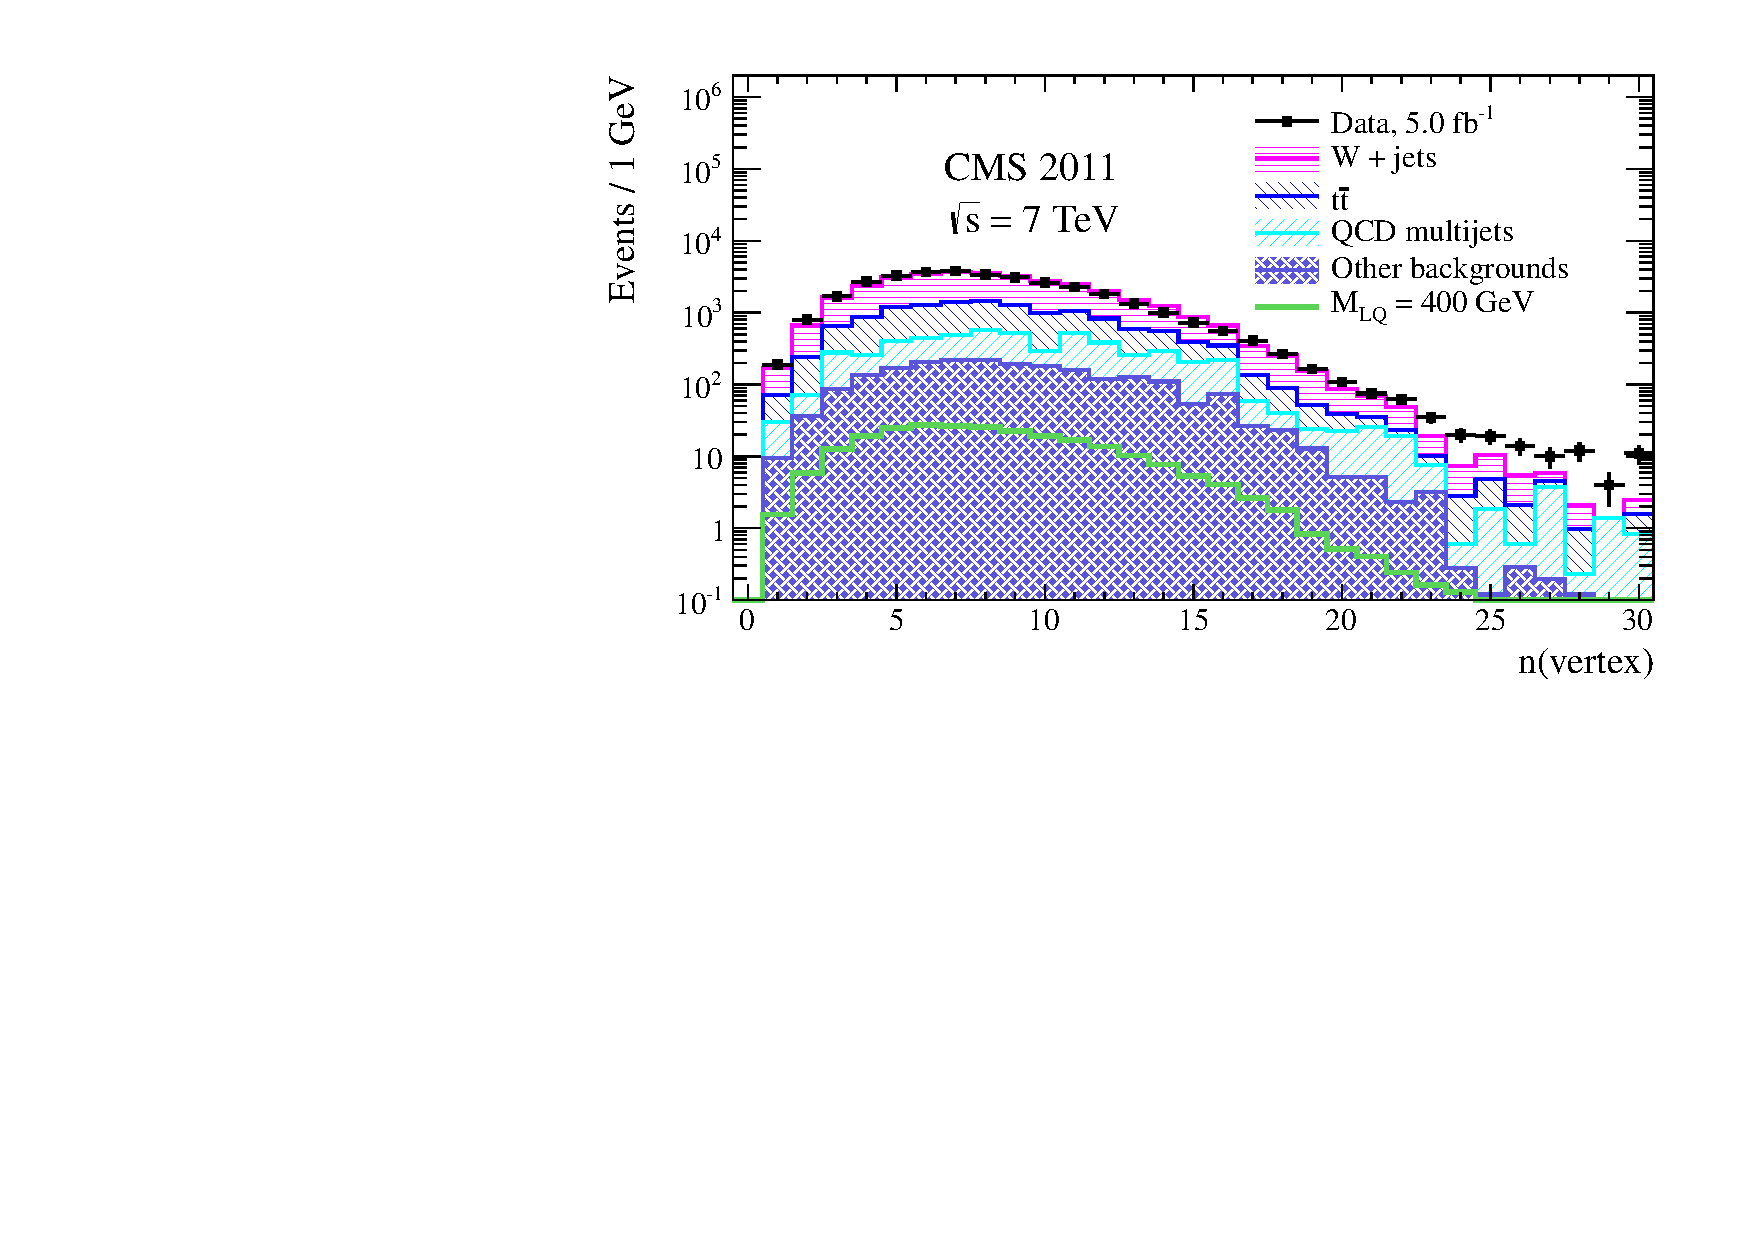
\includegraphics[width=.45\textwidth]{tex/analysis/event_selection/fig/enu/preselection/nVertex_PAS_enujj_WZSherpa_noNSigma.pdf}}\\
    \caption{
      The distribution of the number of primary vertices for events passing the
      \enujj~preselection.
    }
    \label{fig:enujj_preselection_vertices}
  \end{center}
\end{figure*}

\begin{figure*}[htbp]
  \begin{center}
    {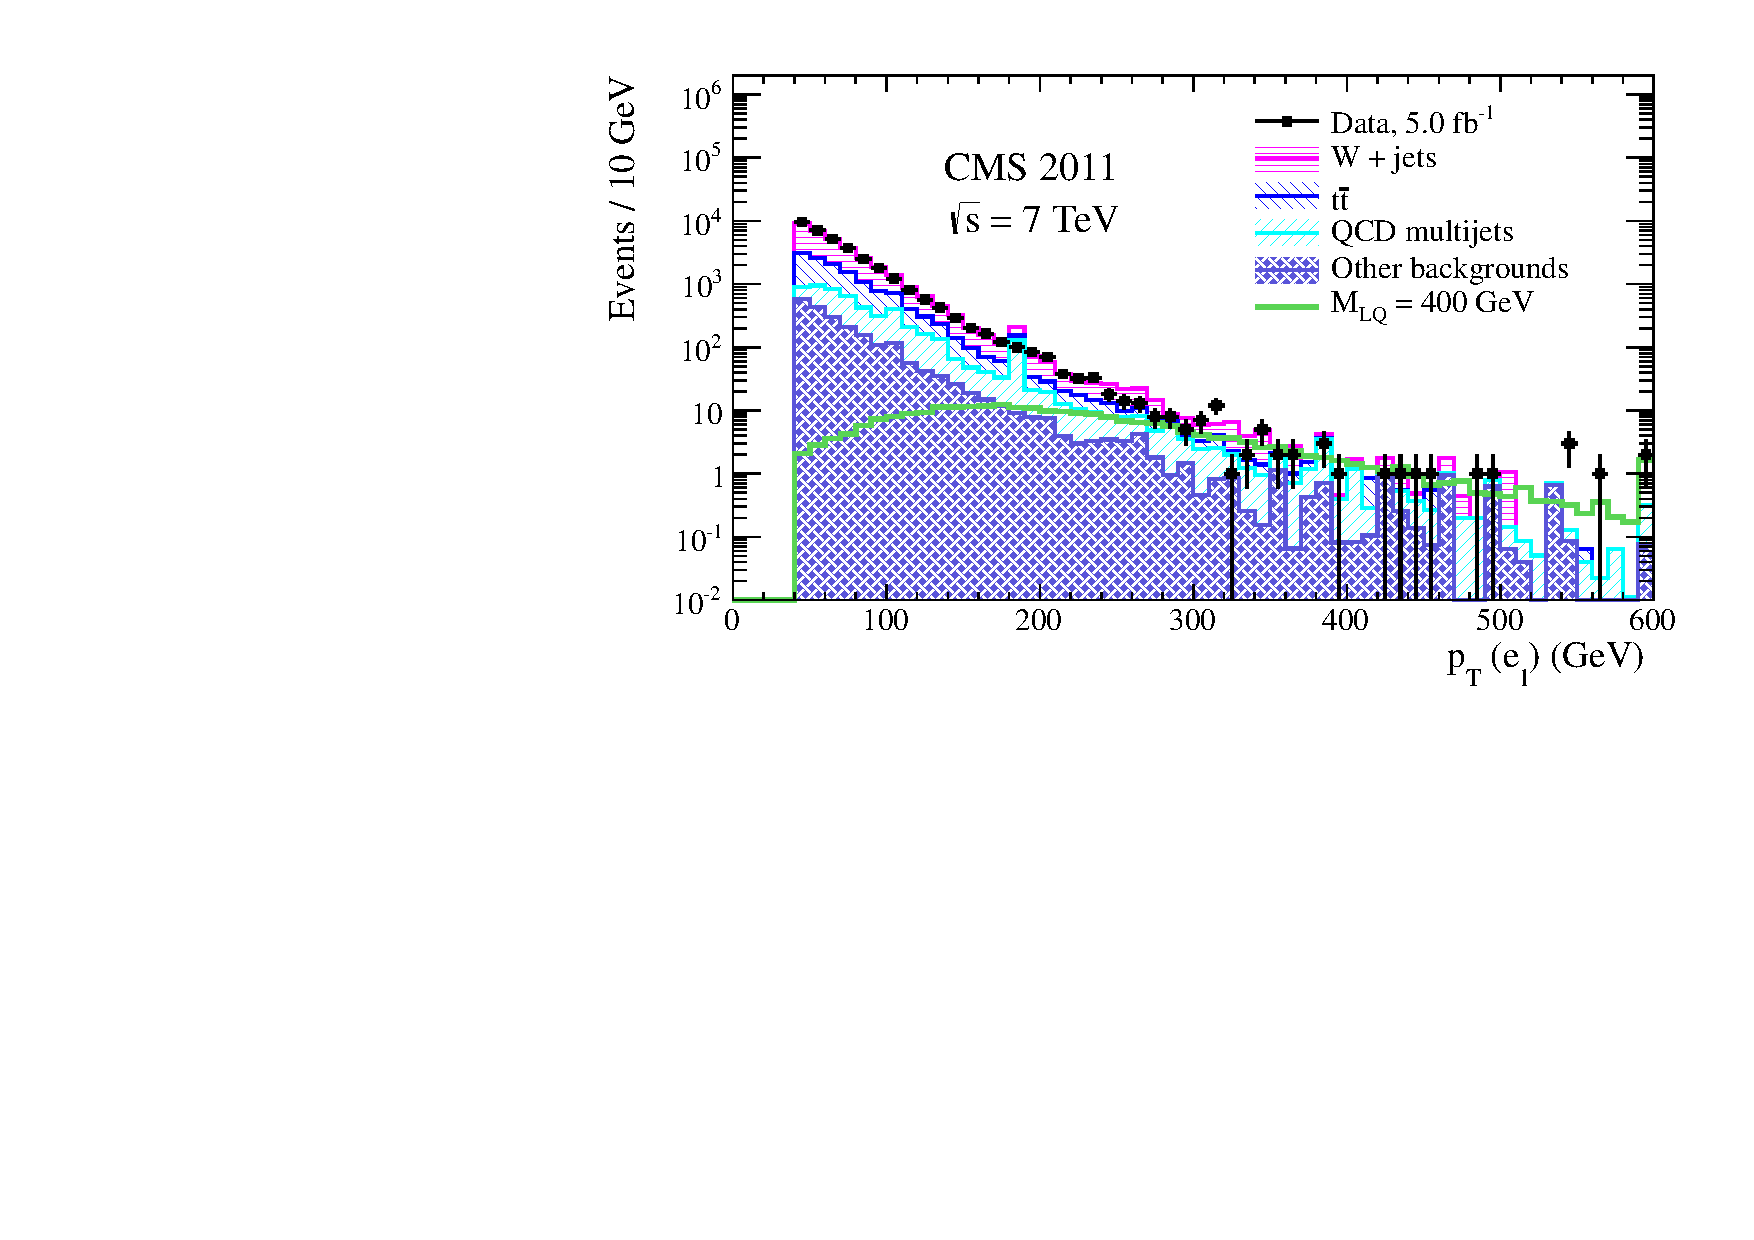
\includegraphics[width=.45\textwidth]{tex/analysis/event_selection/fig/enu/preselection/Pt1stEle_PAS_enujj_WZSherpa_noNSigma.pdf}}
    {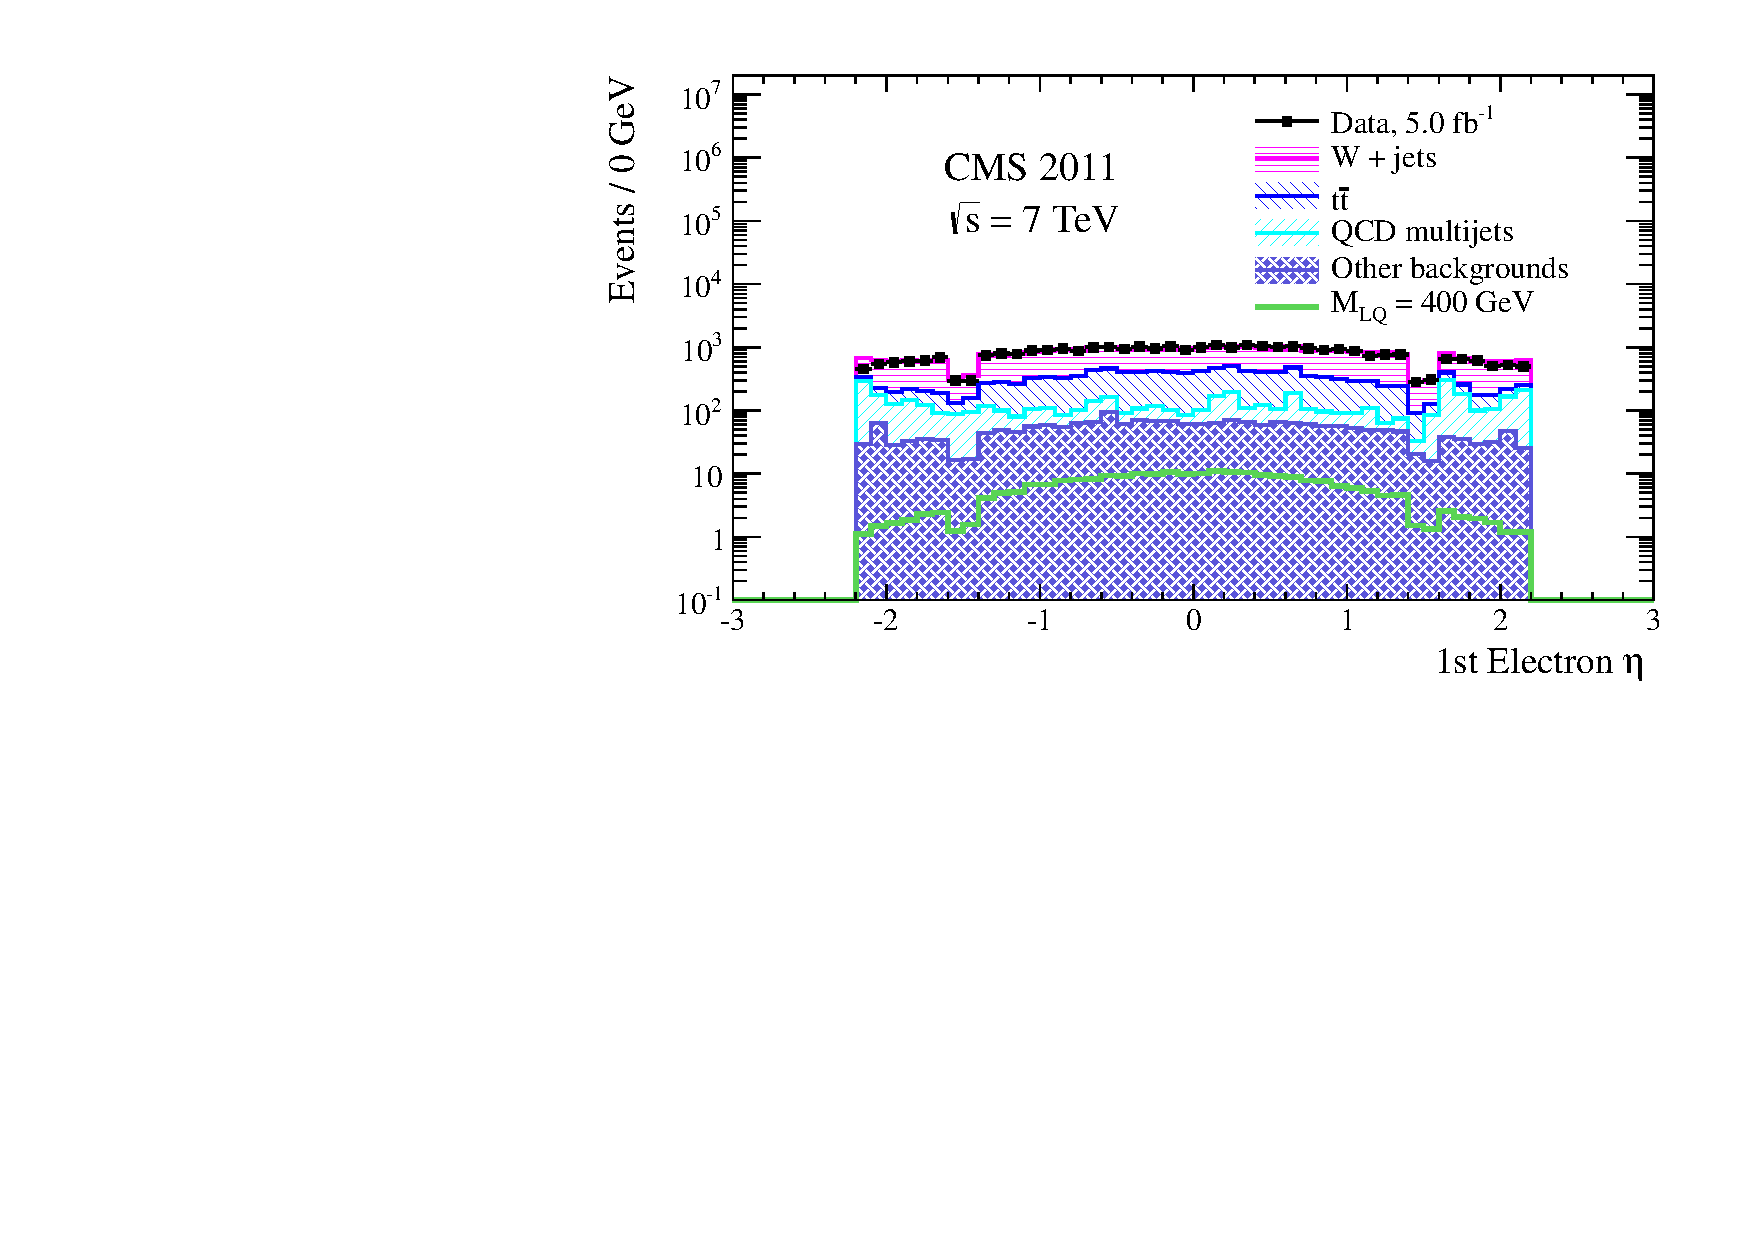
\includegraphics[width=.45\textwidth]{tex/analysis/event_selection/fig/enu/preselection/Eta1stEle_PAS_enujj_WZSherpa_noNSigma.pdf}}
    \caption{
      The \pt (left) and $\eta$ (right) distributions of the leading
      (in \pt) electron for events passing the \enujj~preselection.
    }
    \label{fig:enujj_preselection_ele1}
  \end{center}
\end{figure*}

\begin{figure*}[htbp]
  \begin{center}
    {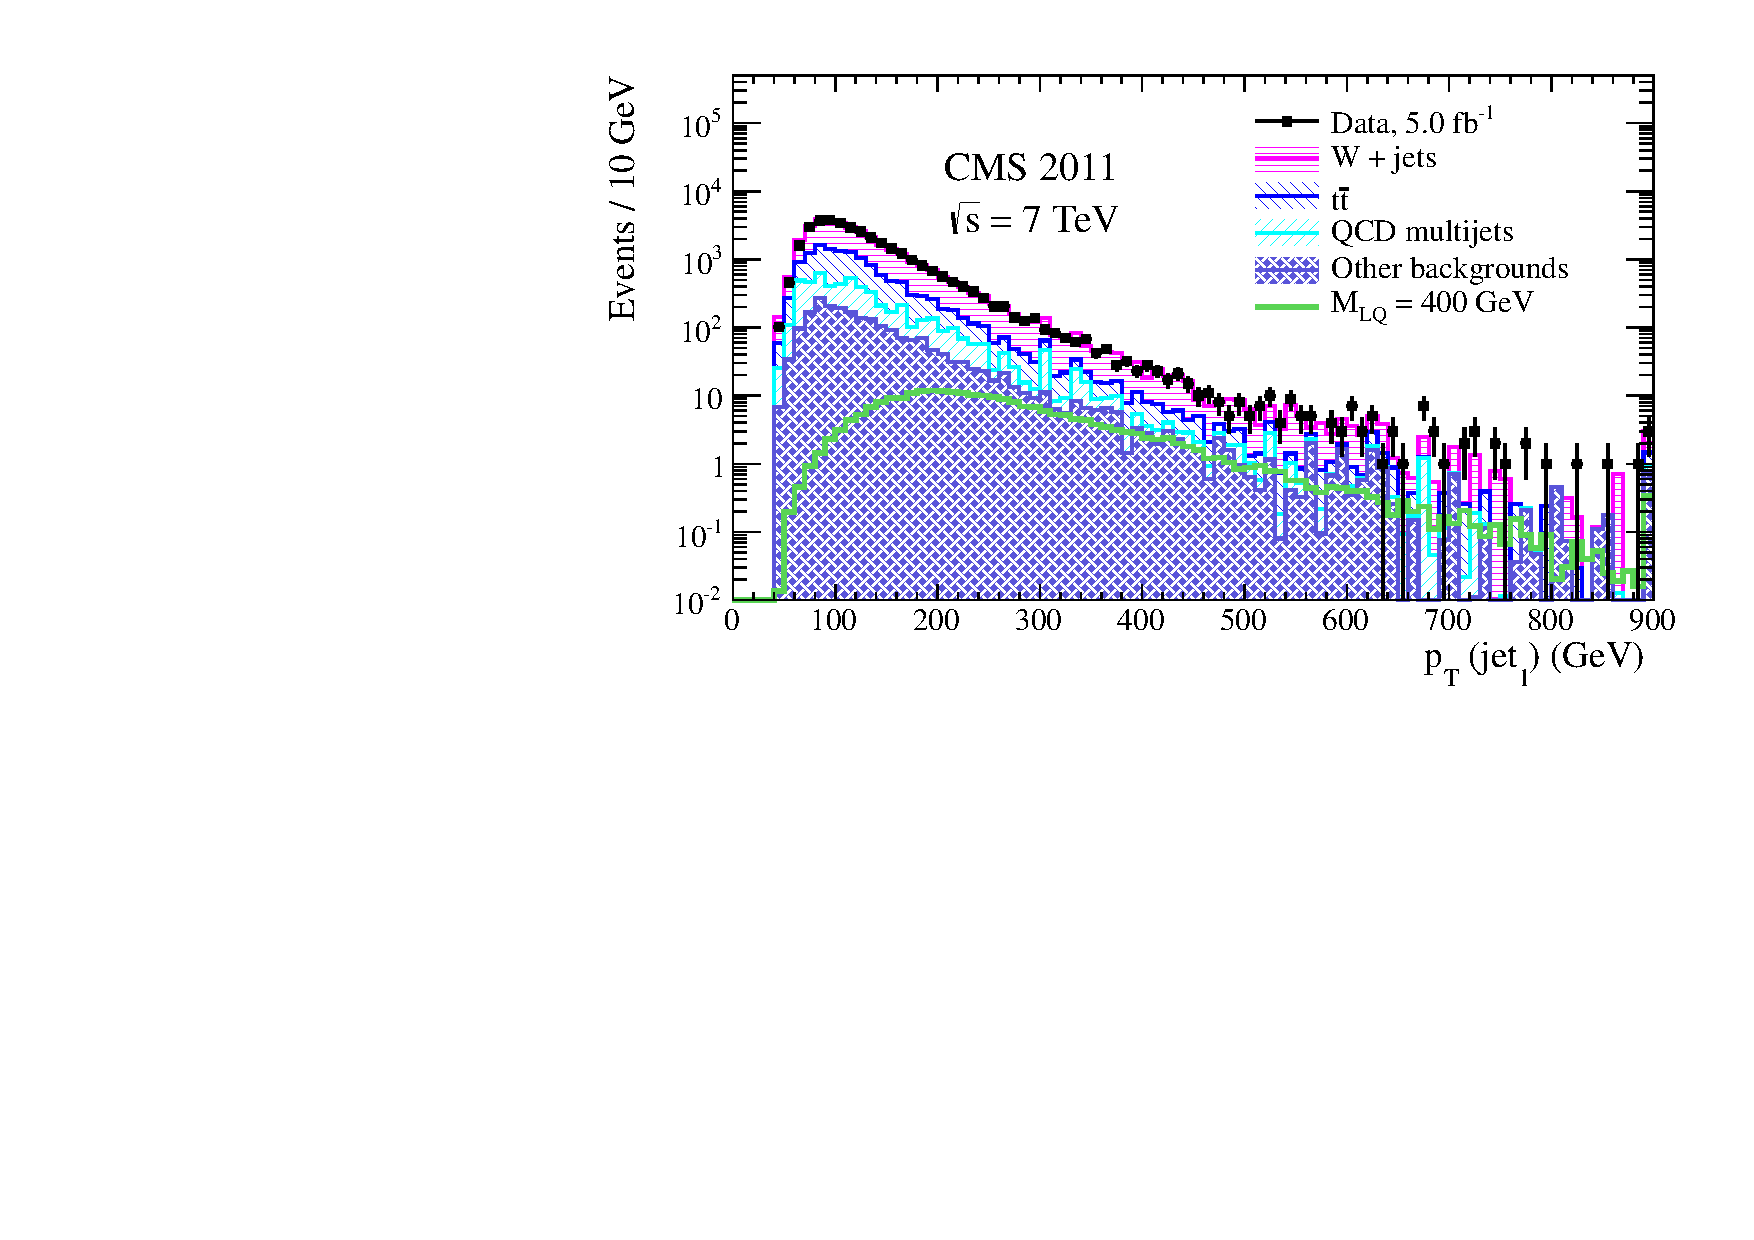
\includegraphics[width=.45\textwidth]{tex/analysis/event_selection/fig/enu/preselection/Pt1stJet_PAS_enujj_WZSherpa_noNSigma.pdf}}
    {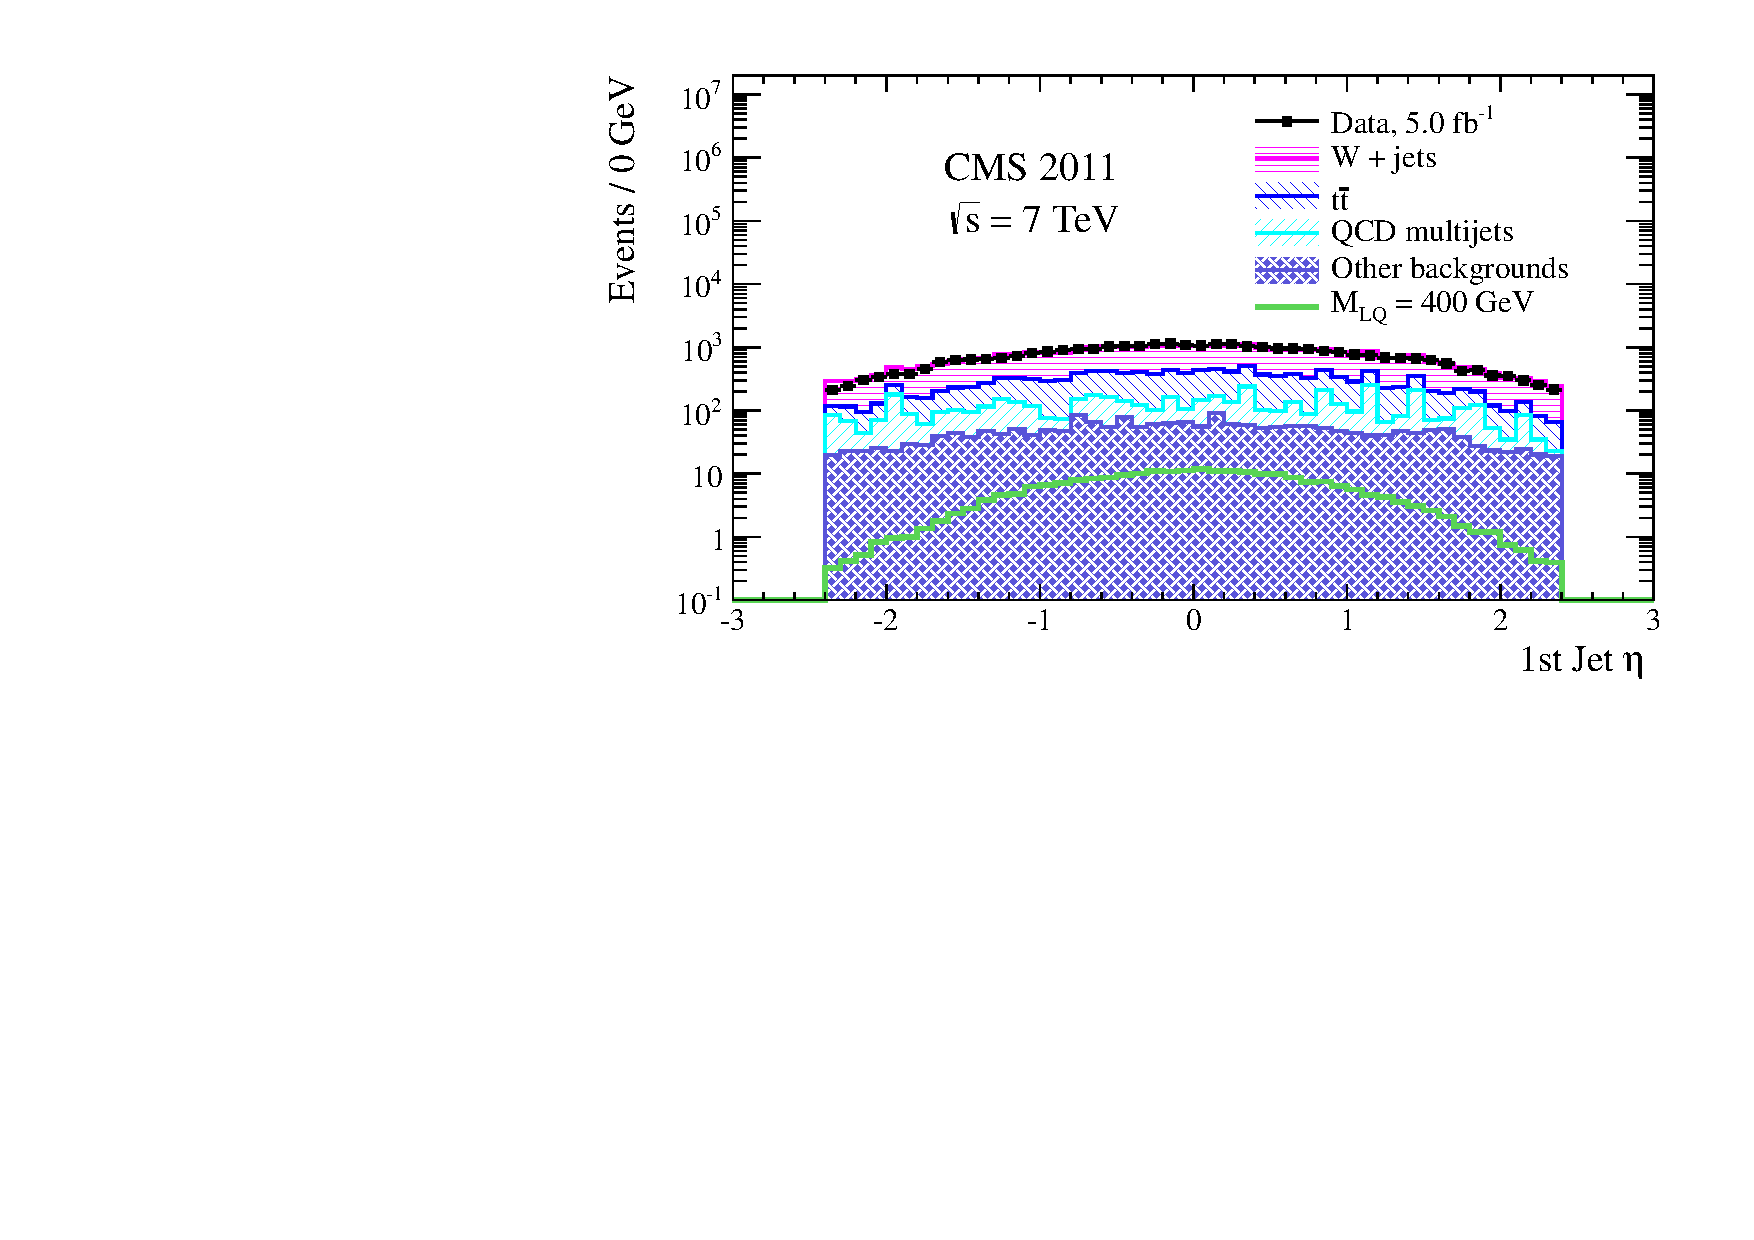
\includegraphics[width=.45\textwidth]{tex/analysis/event_selection/fig/enu/preselection/Eta1stJet_PAS_enujj_WZSherpa_noNSigma.pdf}}
    \caption{
      The \pt (left) and $\eta$ (right) distributions of the leading
      (in \pt) jet for events passing the \enujj~preselection.
    }
    \label{fig:enujj_preselection_jet1}
  \end{center}
\end{figure*}

\begin{figure*}[htbp]
  \begin{center}
    {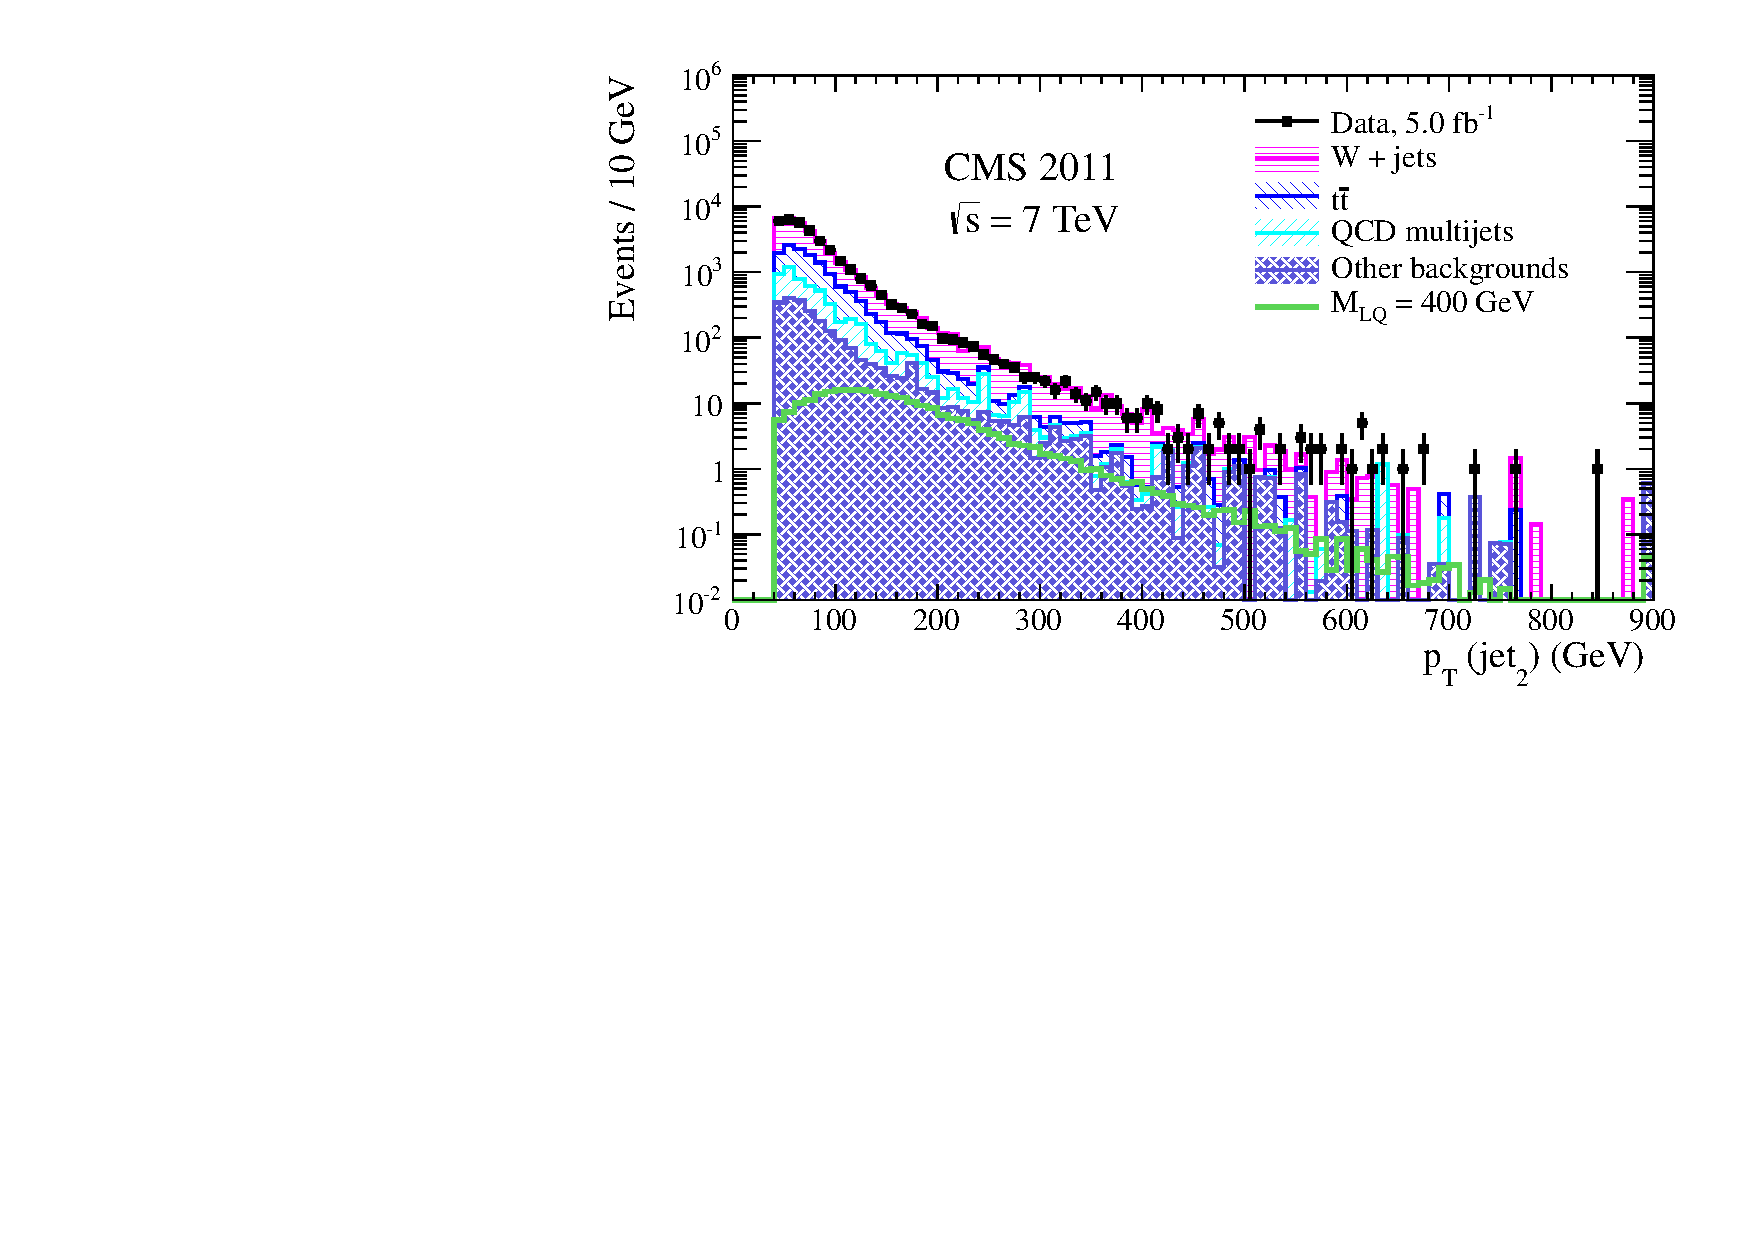
\includegraphics[width=.45\textwidth]{tex/analysis/event_selection/fig/enu/preselection/Pt2ndJet_PAS_enujj_WZSherpa_noNSigma.pdf}}
    {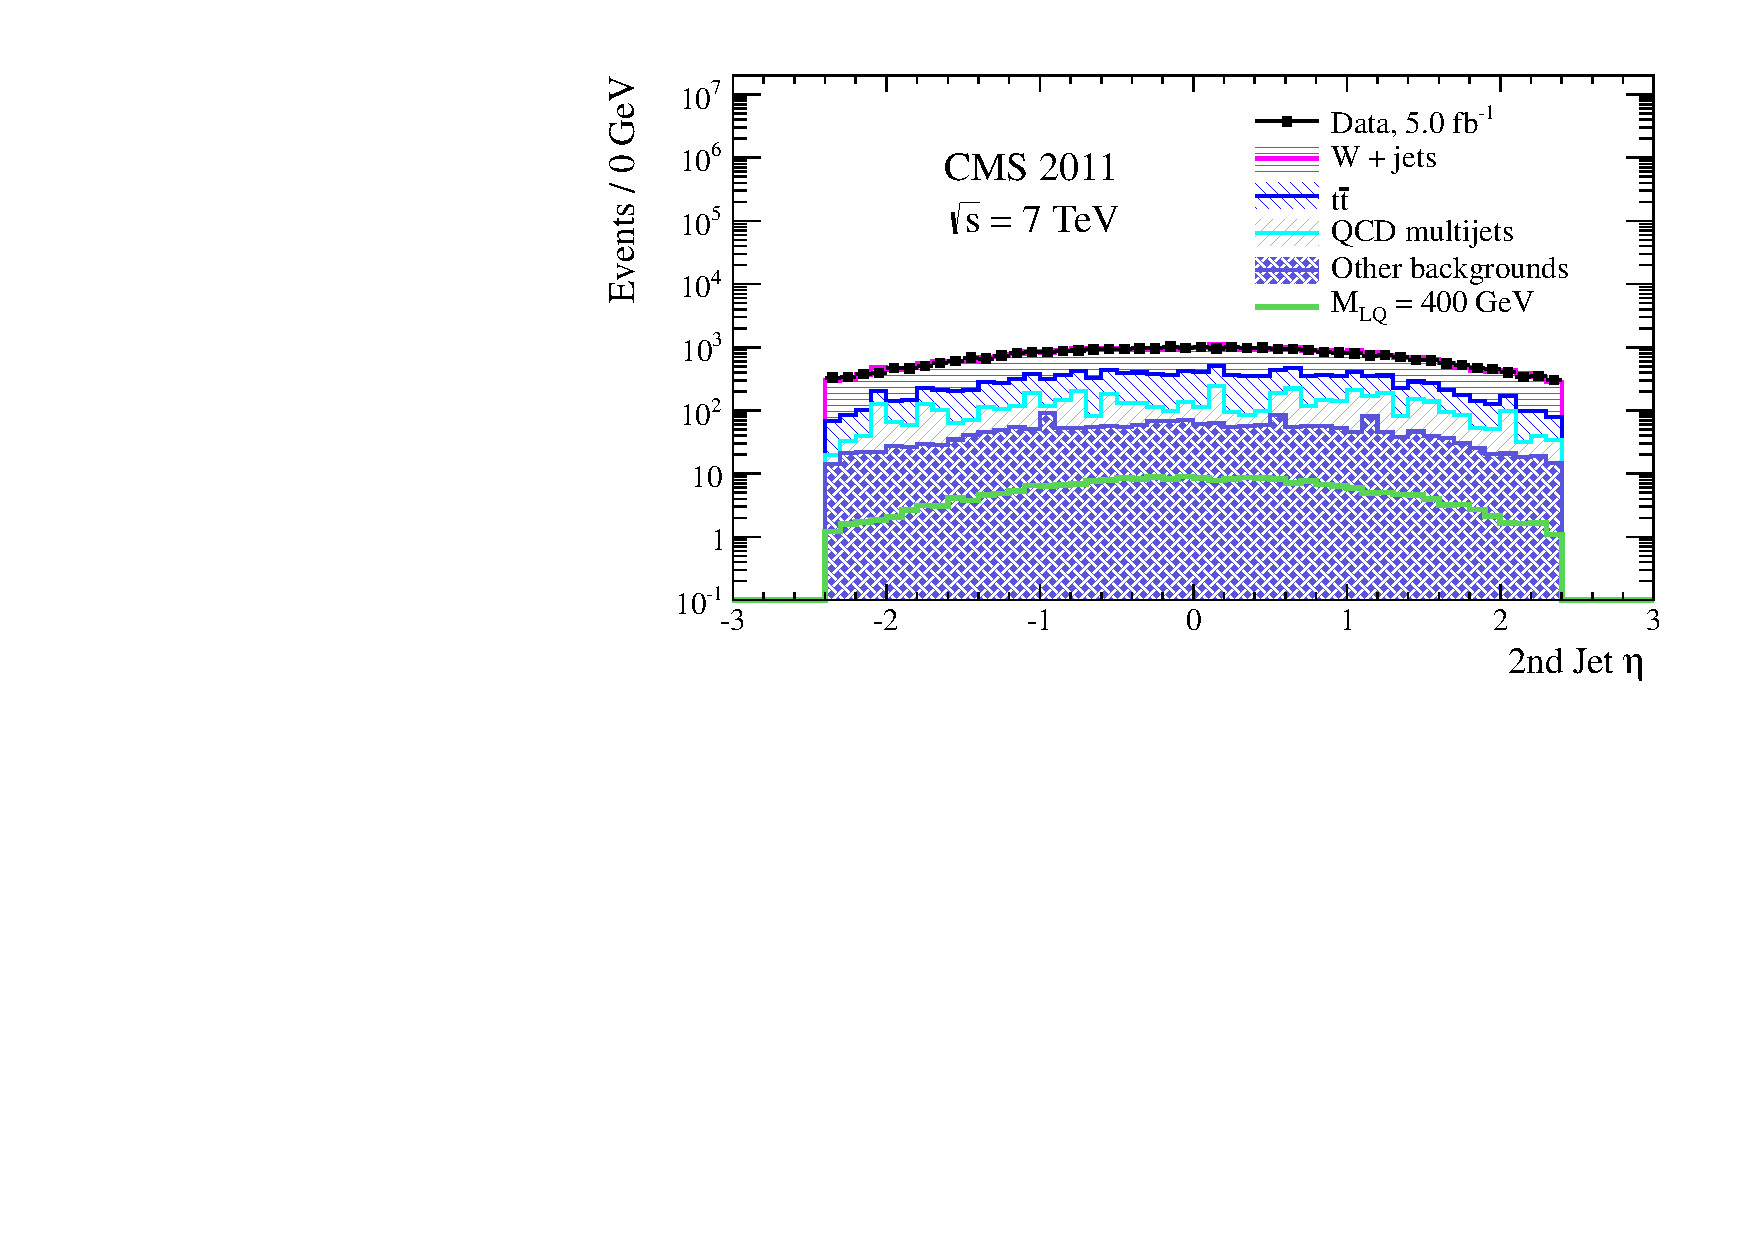
\includegraphics[width=.45\textwidth]{tex/analysis/event_selection/fig/enu/preselection/Eta2ndJet_PAS_enujj_WZSherpa_noNSigma.pdf}}
    \caption{
      The \pt (left) and $\eta$ (right) distributions of the second leading
      (in \pt) jet for events passing the \enujj~preselection.
    }
    \label{fig:enujj_preselection_jet2}
  \end{center}
\end{figure*}

\begin{figure*}[htbp]
  \begin{center}
    {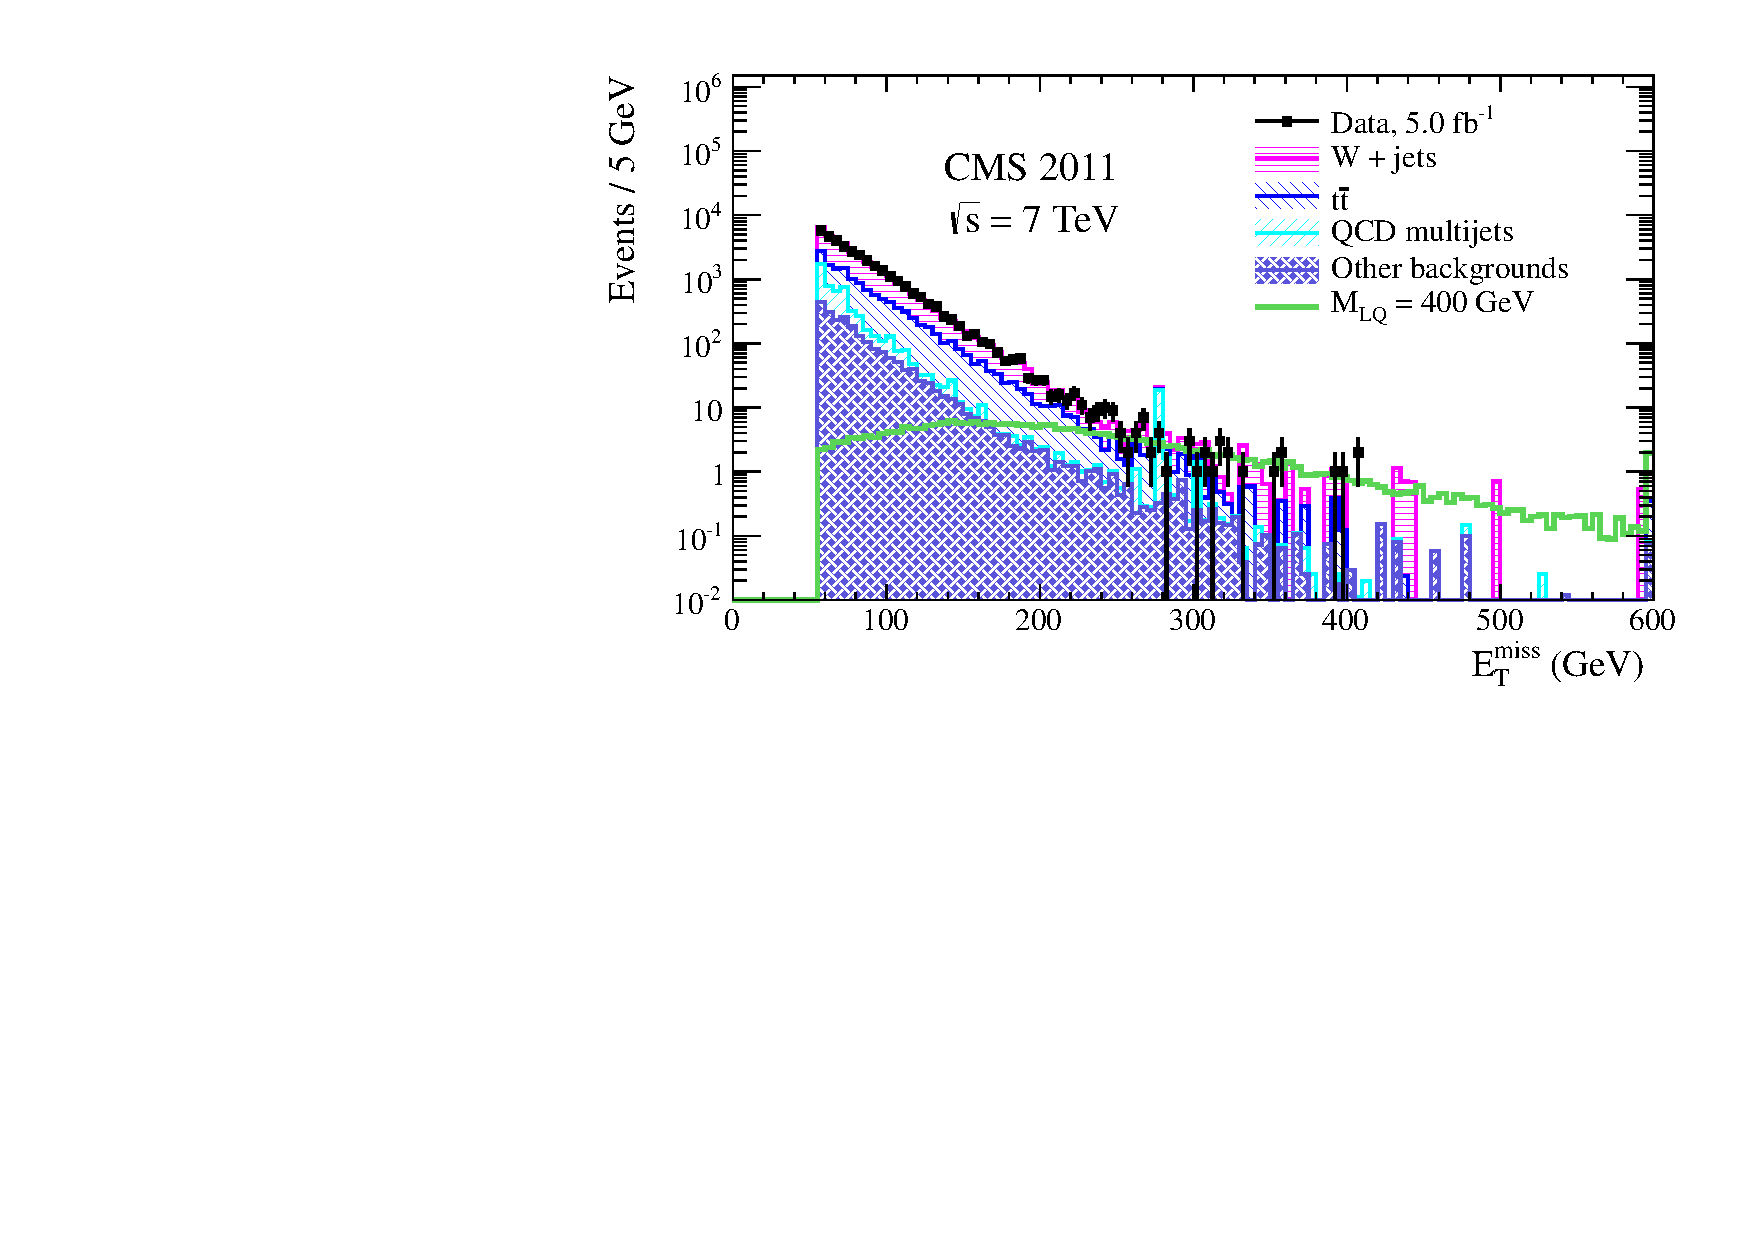
\includegraphics[width=.45\textwidth]{tex/analysis/event_selection/fig/enu/preselection/MET_PAS_enujj_WZSherpa_noNSigma.pdf}}
    {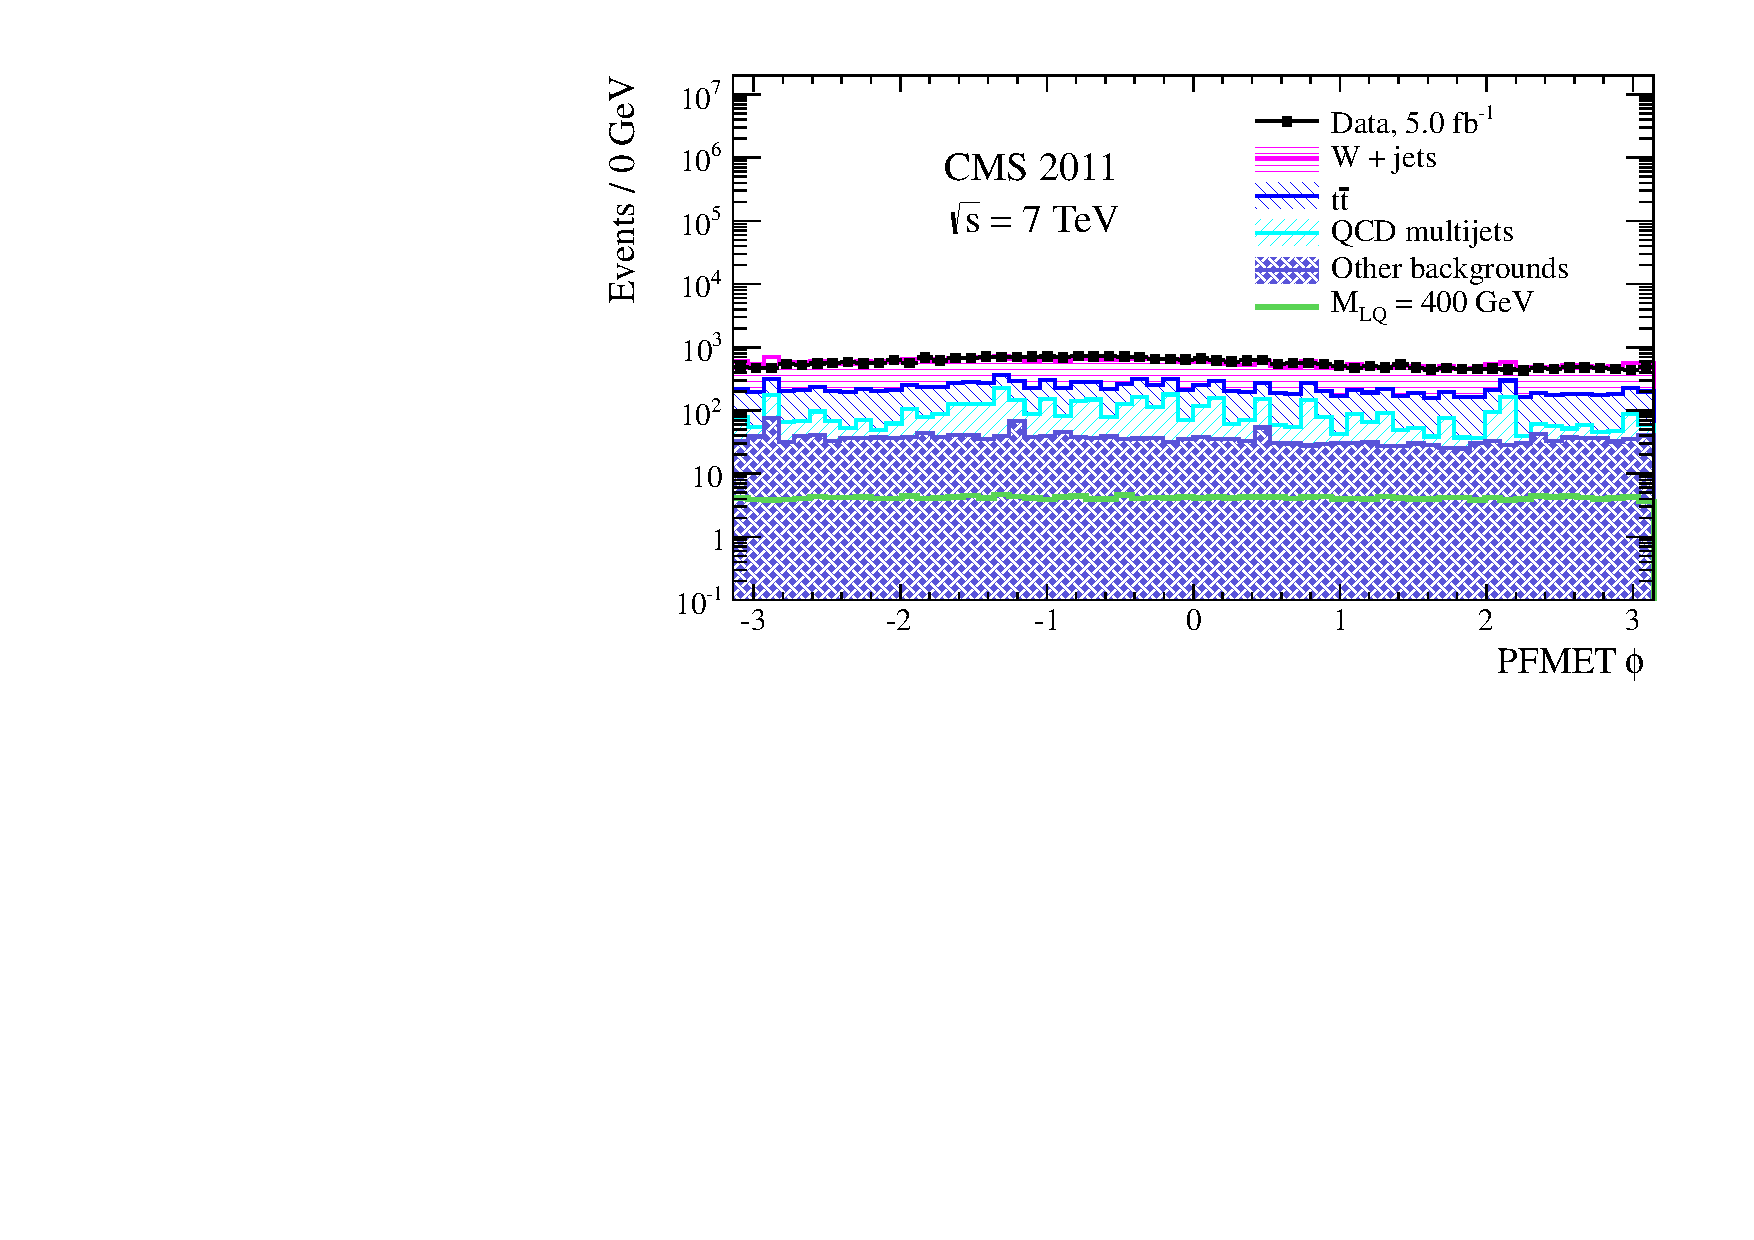
\includegraphics[width=.45\textwidth]{tex/analysis/event_selection/fig/enu/preselection/METPhi_PAS_enujj_WZSherpa_noNSigma.pdf}}
    \caption{
      The \MET (left) and $\phi(\MET)$ (right) distributions for events passing the \enujj~preselection.
    }
    \label{fig:enujj_preselection_met}
  \end{center}
\end{figure*}

\begin{figure*}[htbp]
  \begin{center}
    {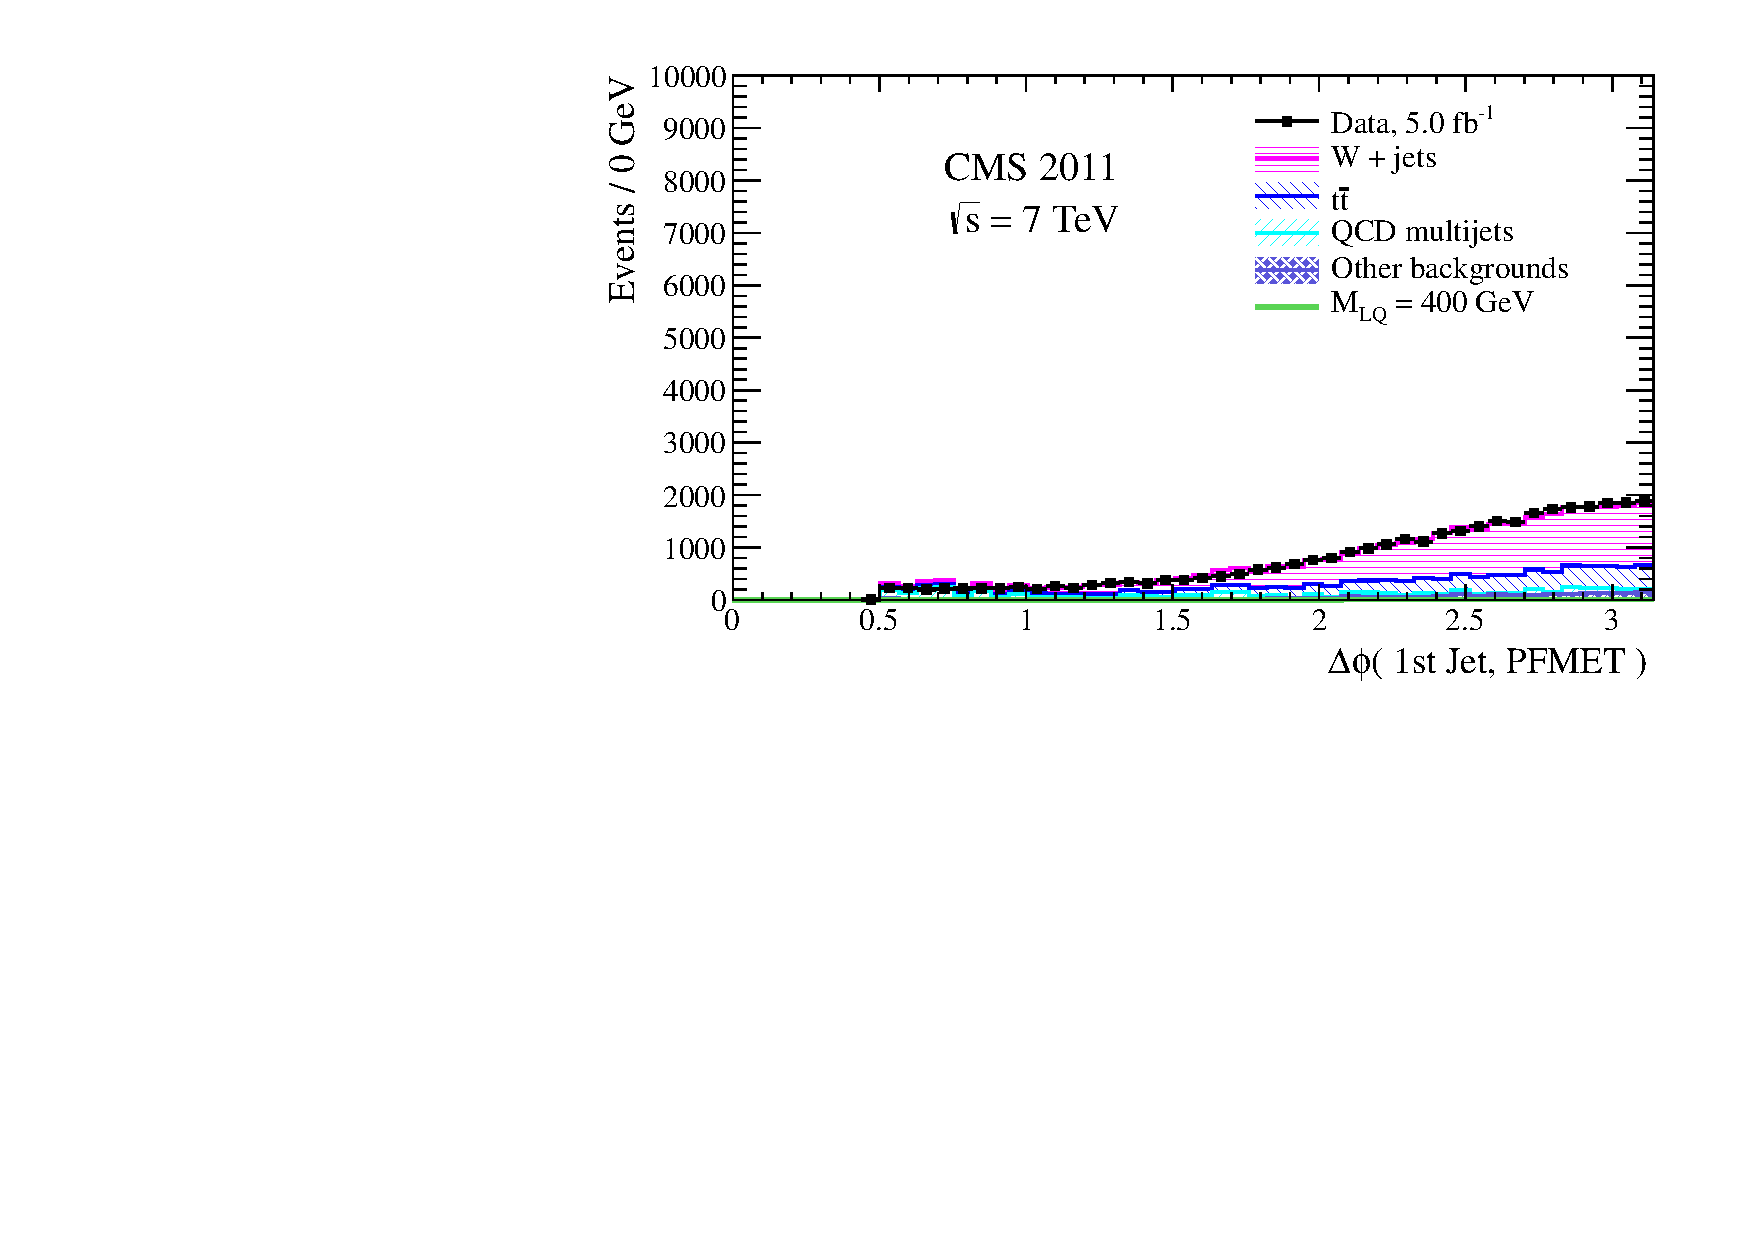
\includegraphics[width=.45\textwidth]{tex/analysis/event_selection/fig/enu/preselection/mDPhi1stJetMET_PAS_enujj_WZSherpa_noNSigma.pdf}}
    {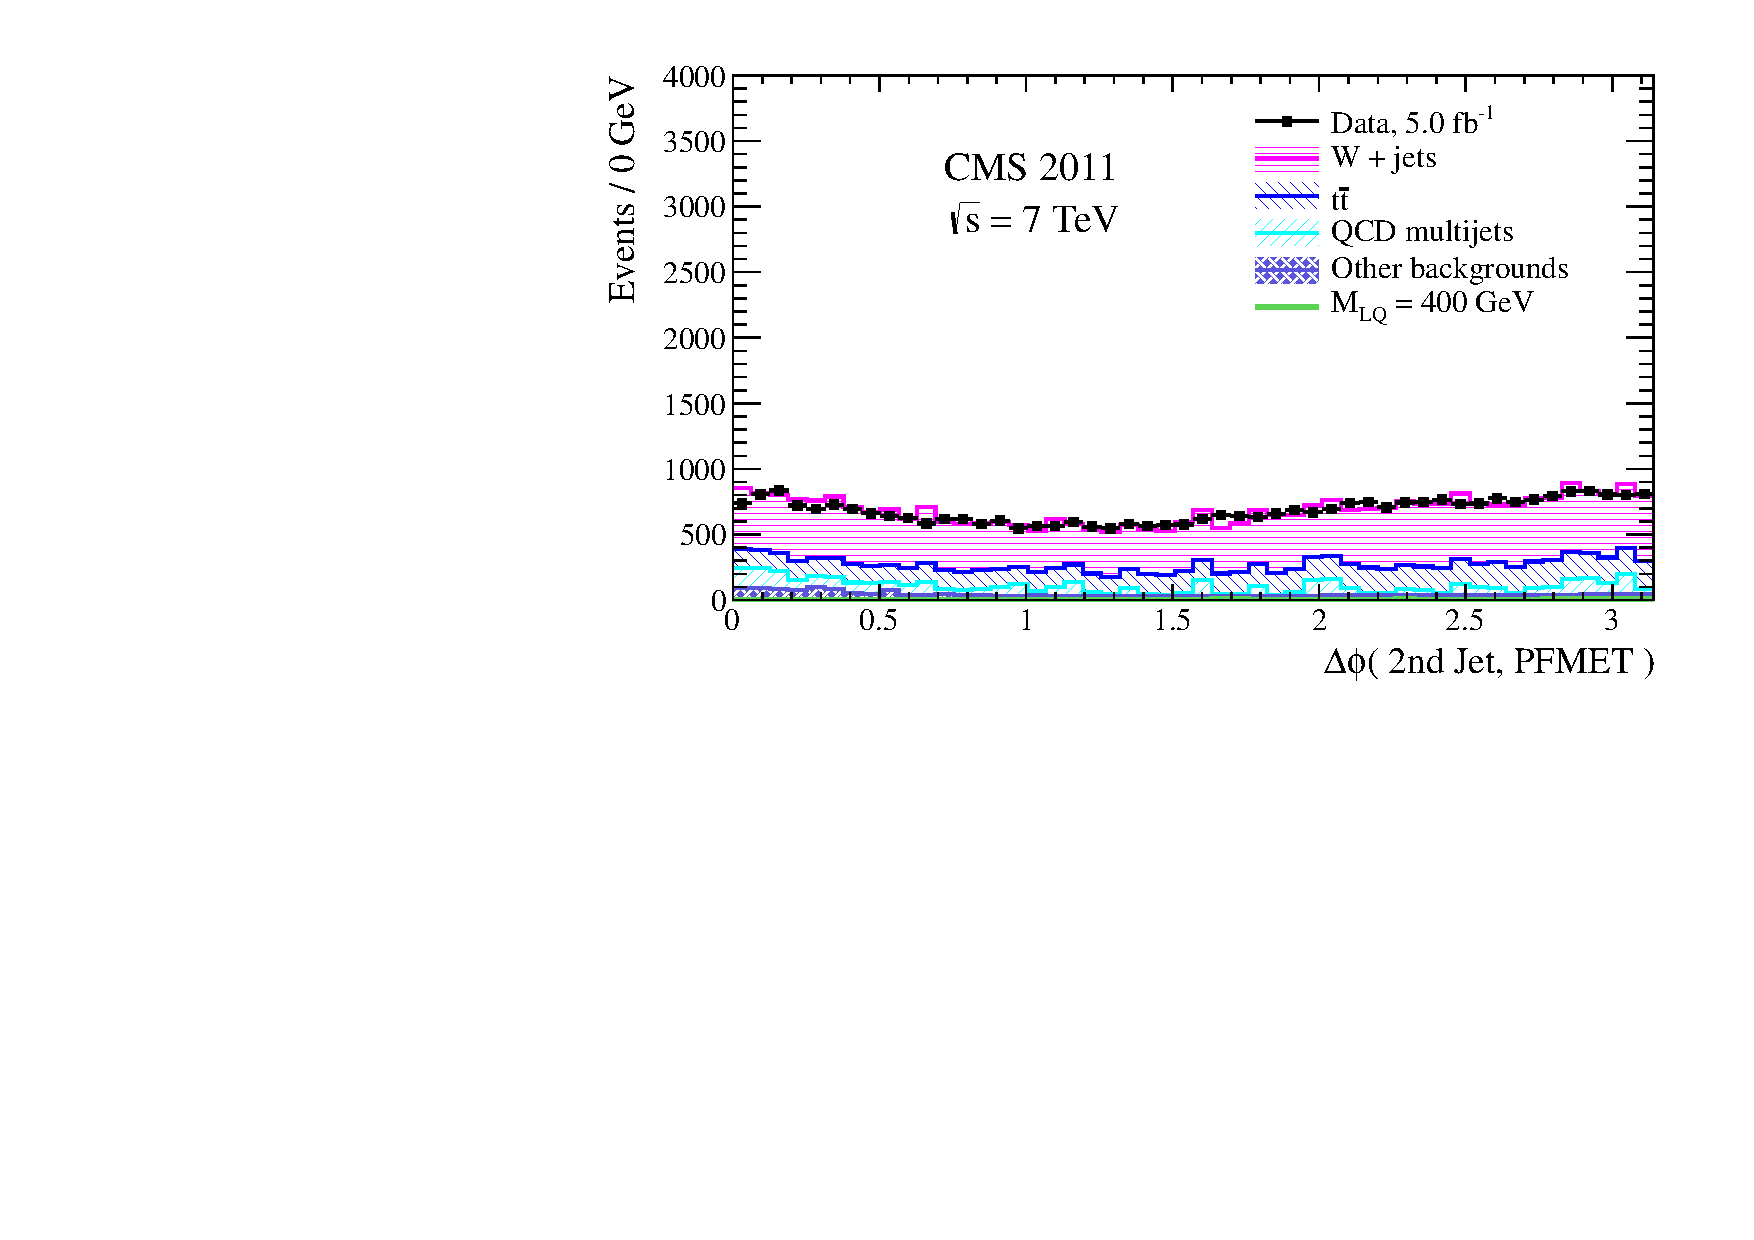
\includegraphics[width=.45\textwidth]{tex/analysis/event_selection/fig/enu/preselection/mDPhi2ndJetMET_PAS_enujj_WZSherpa_noNSigma.pdf}} \\
    {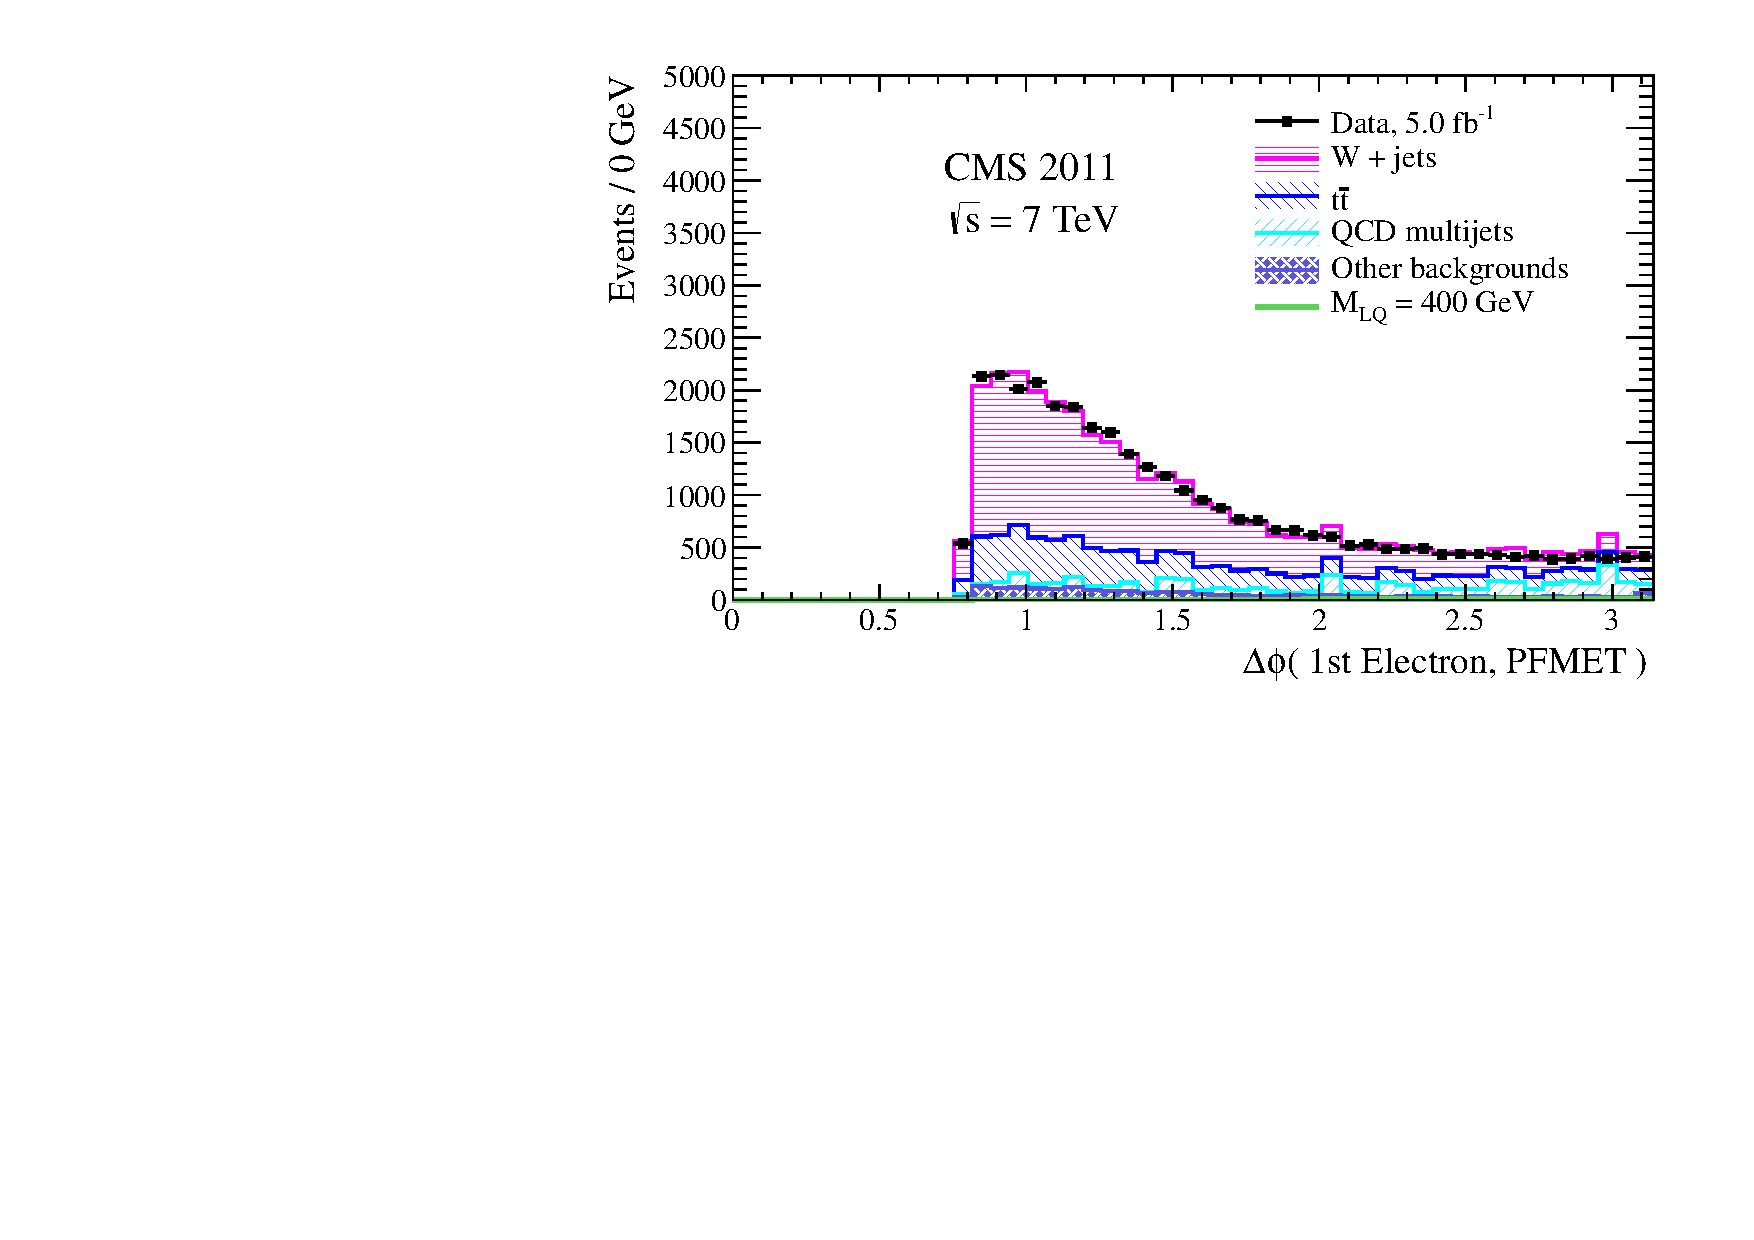
\includegraphics[width=.45\textwidth]{tex/analysis/event_selection/fig/enu/preselection/mDPhi1stEleMET_PAS_enujj_WZSherpa_noNSigma.pdf}}
    {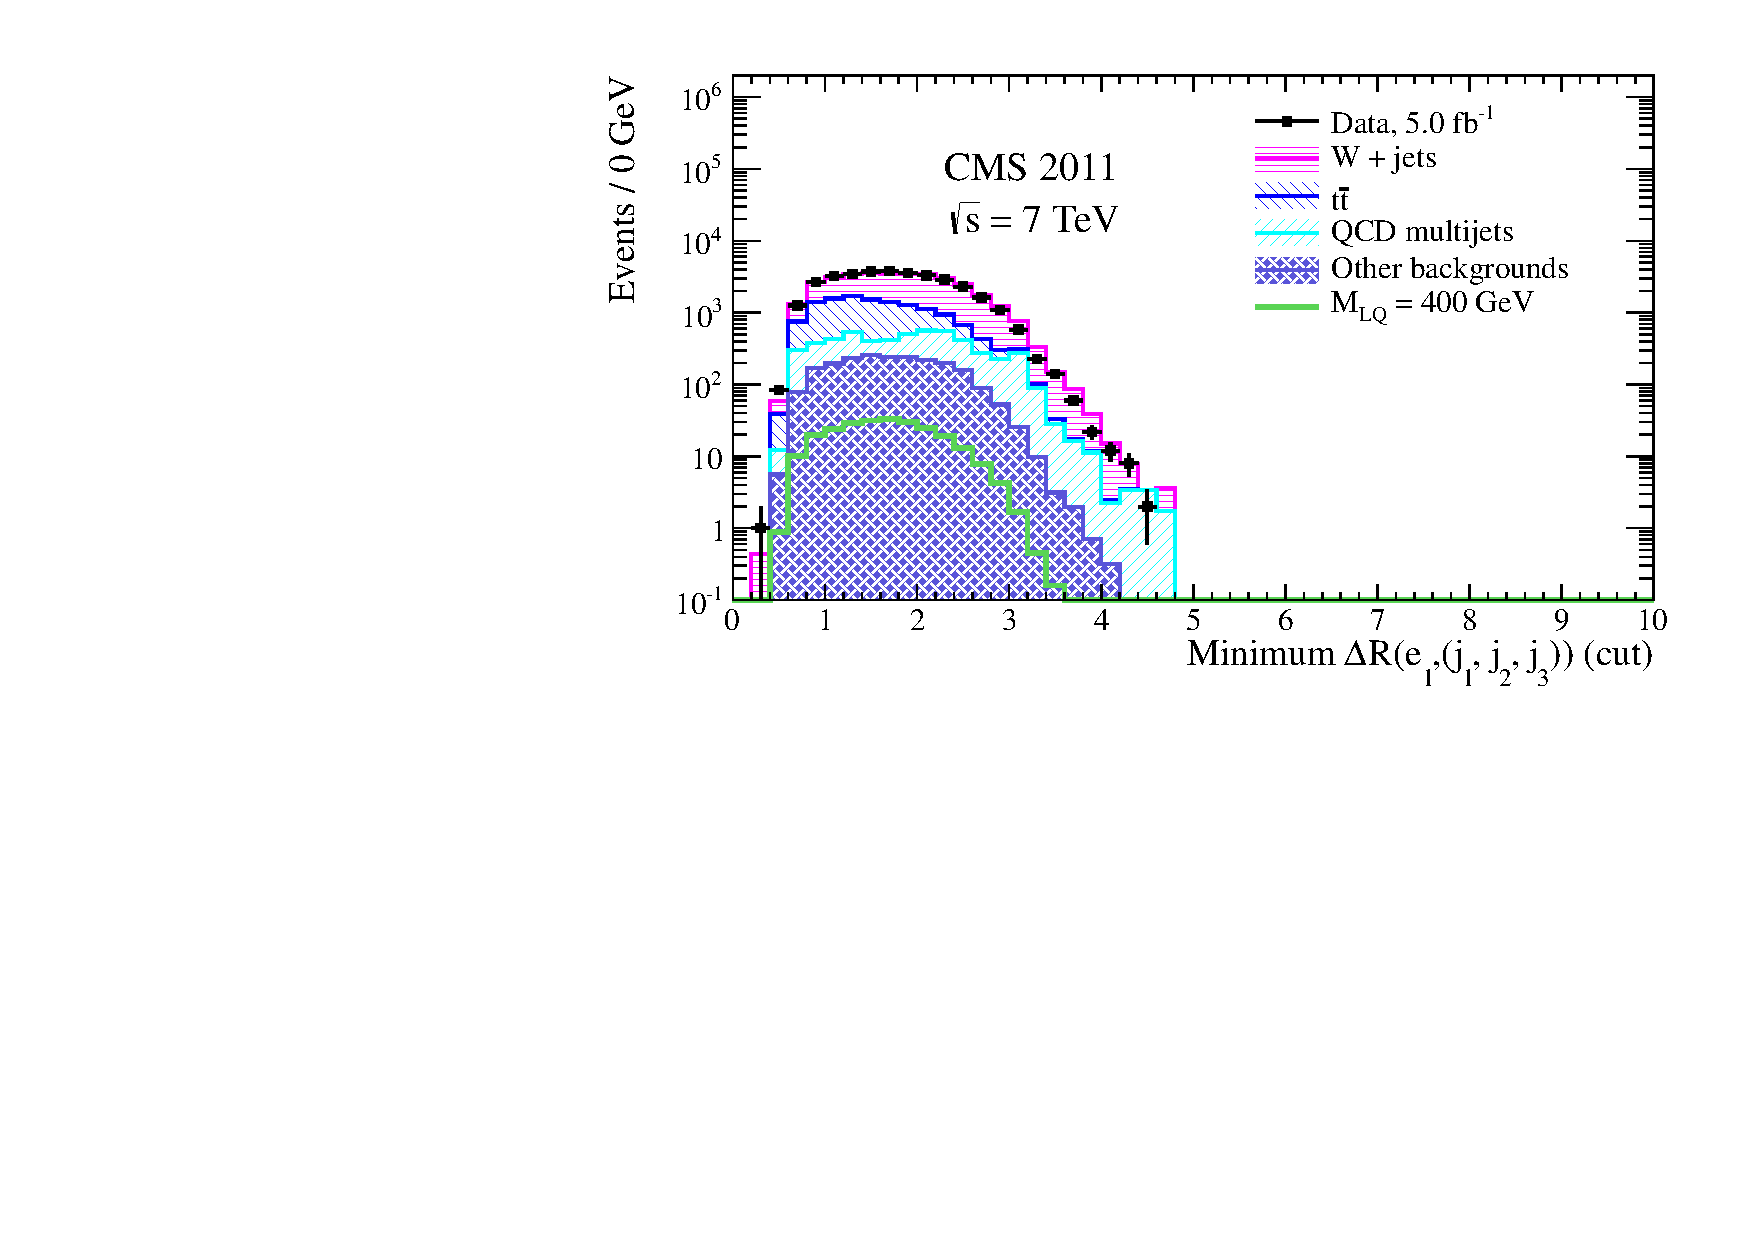
\includegraphics[width=.45\textwidth]{tex/analysis/event_selection/fig/enu/preselection/minDR_EleJet_PAS_enujj_WZSherpa_noNSigma.pdf}}
    \caption{
      The distribution of 
      $\Delta|phi(\MET,\text{j1})$ (top left), 
      $\Delta|phi(\MET,\text{j2})$ (top right),
      $\Delta|phi(\MET,\text{e})$  (bottom left), and 
      $\text{min}\Delta R (\text{e},\text{jets})$ (bottom right)
      for events passing the \enujj~preselection.
    }
    \label{fig:enujj_preselection_deltaPhi}
  \end{center}
\end{figure*}

\begin{figure*}[htbp]
  \begin{center}
    {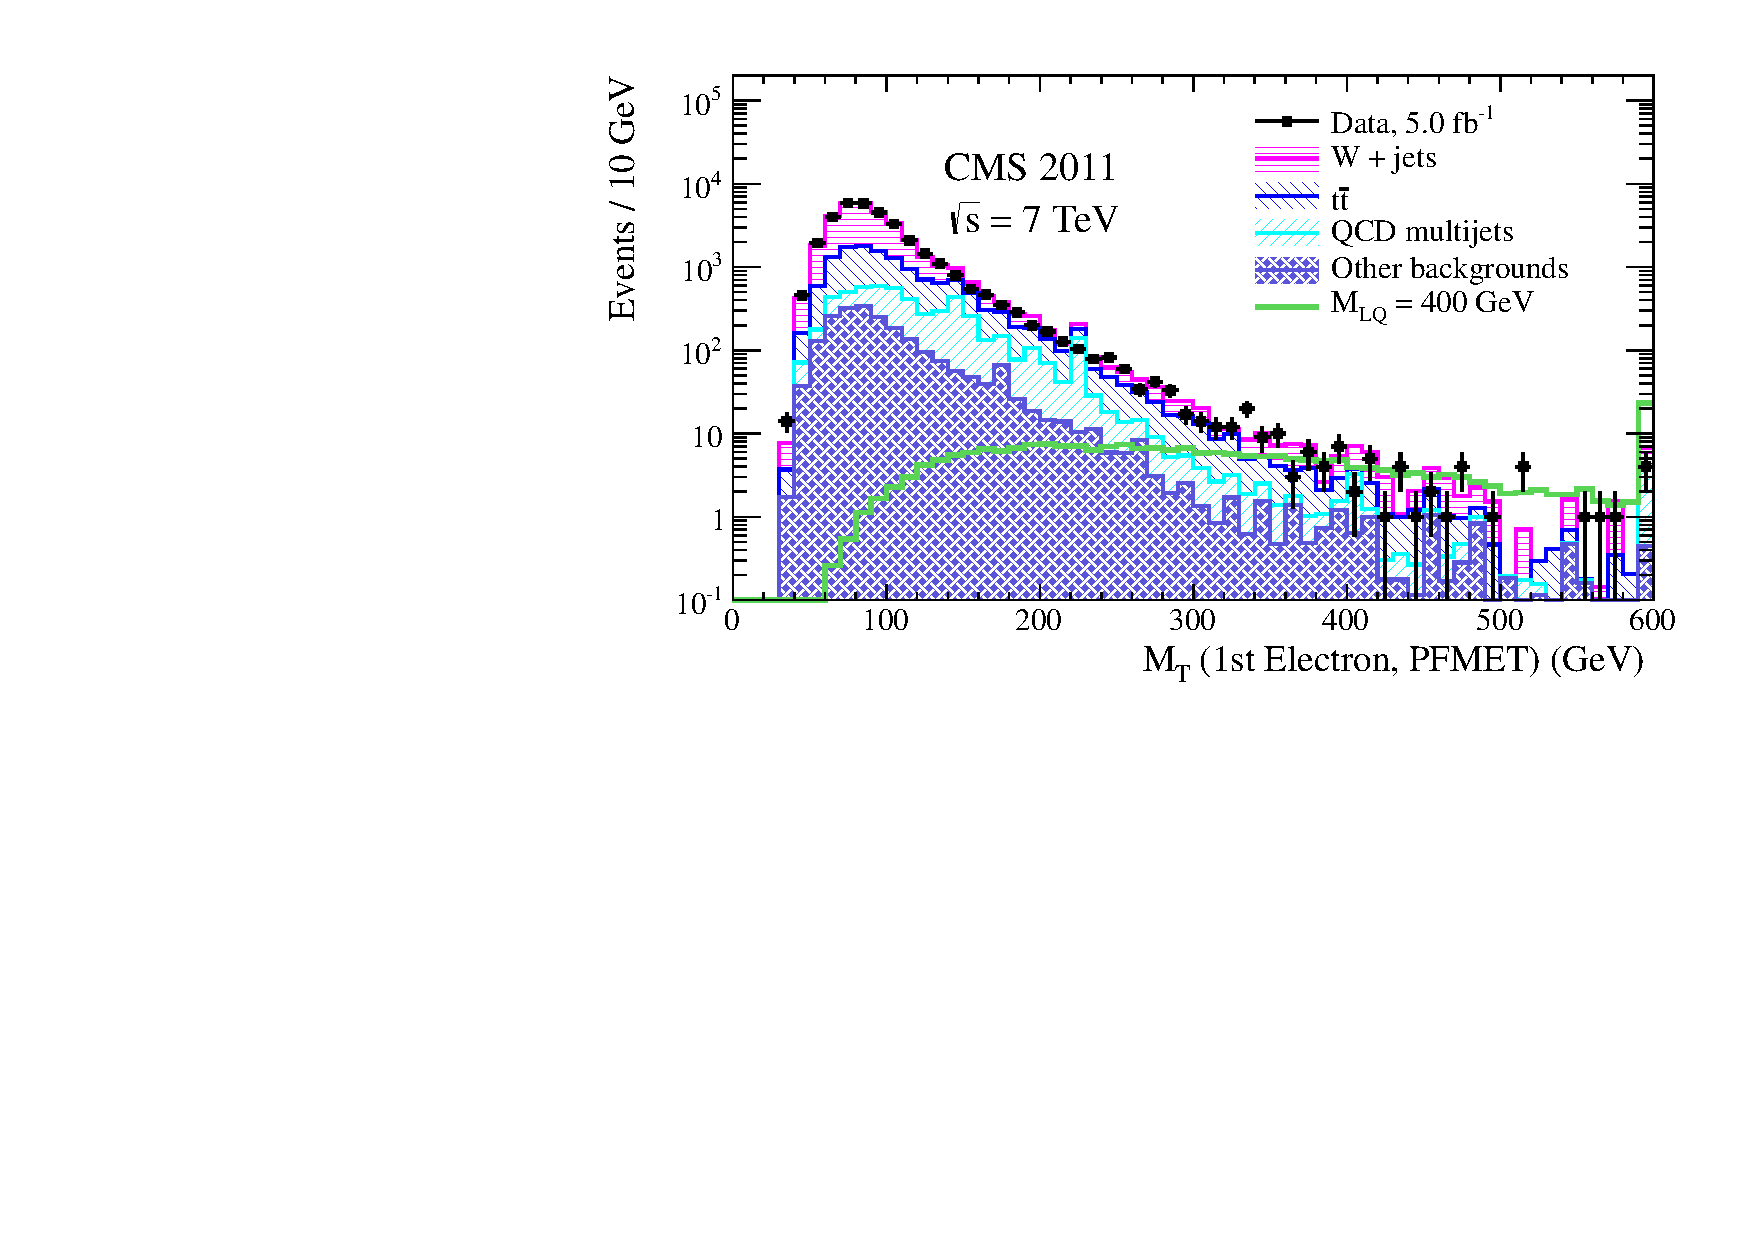
\includegraphics[width=.45\textwidth]{tex/analysis/event_selection/fig/enu/preselection/MTenu_PAS_enujj_WZSherpa_noNSigma.pdf}}
    {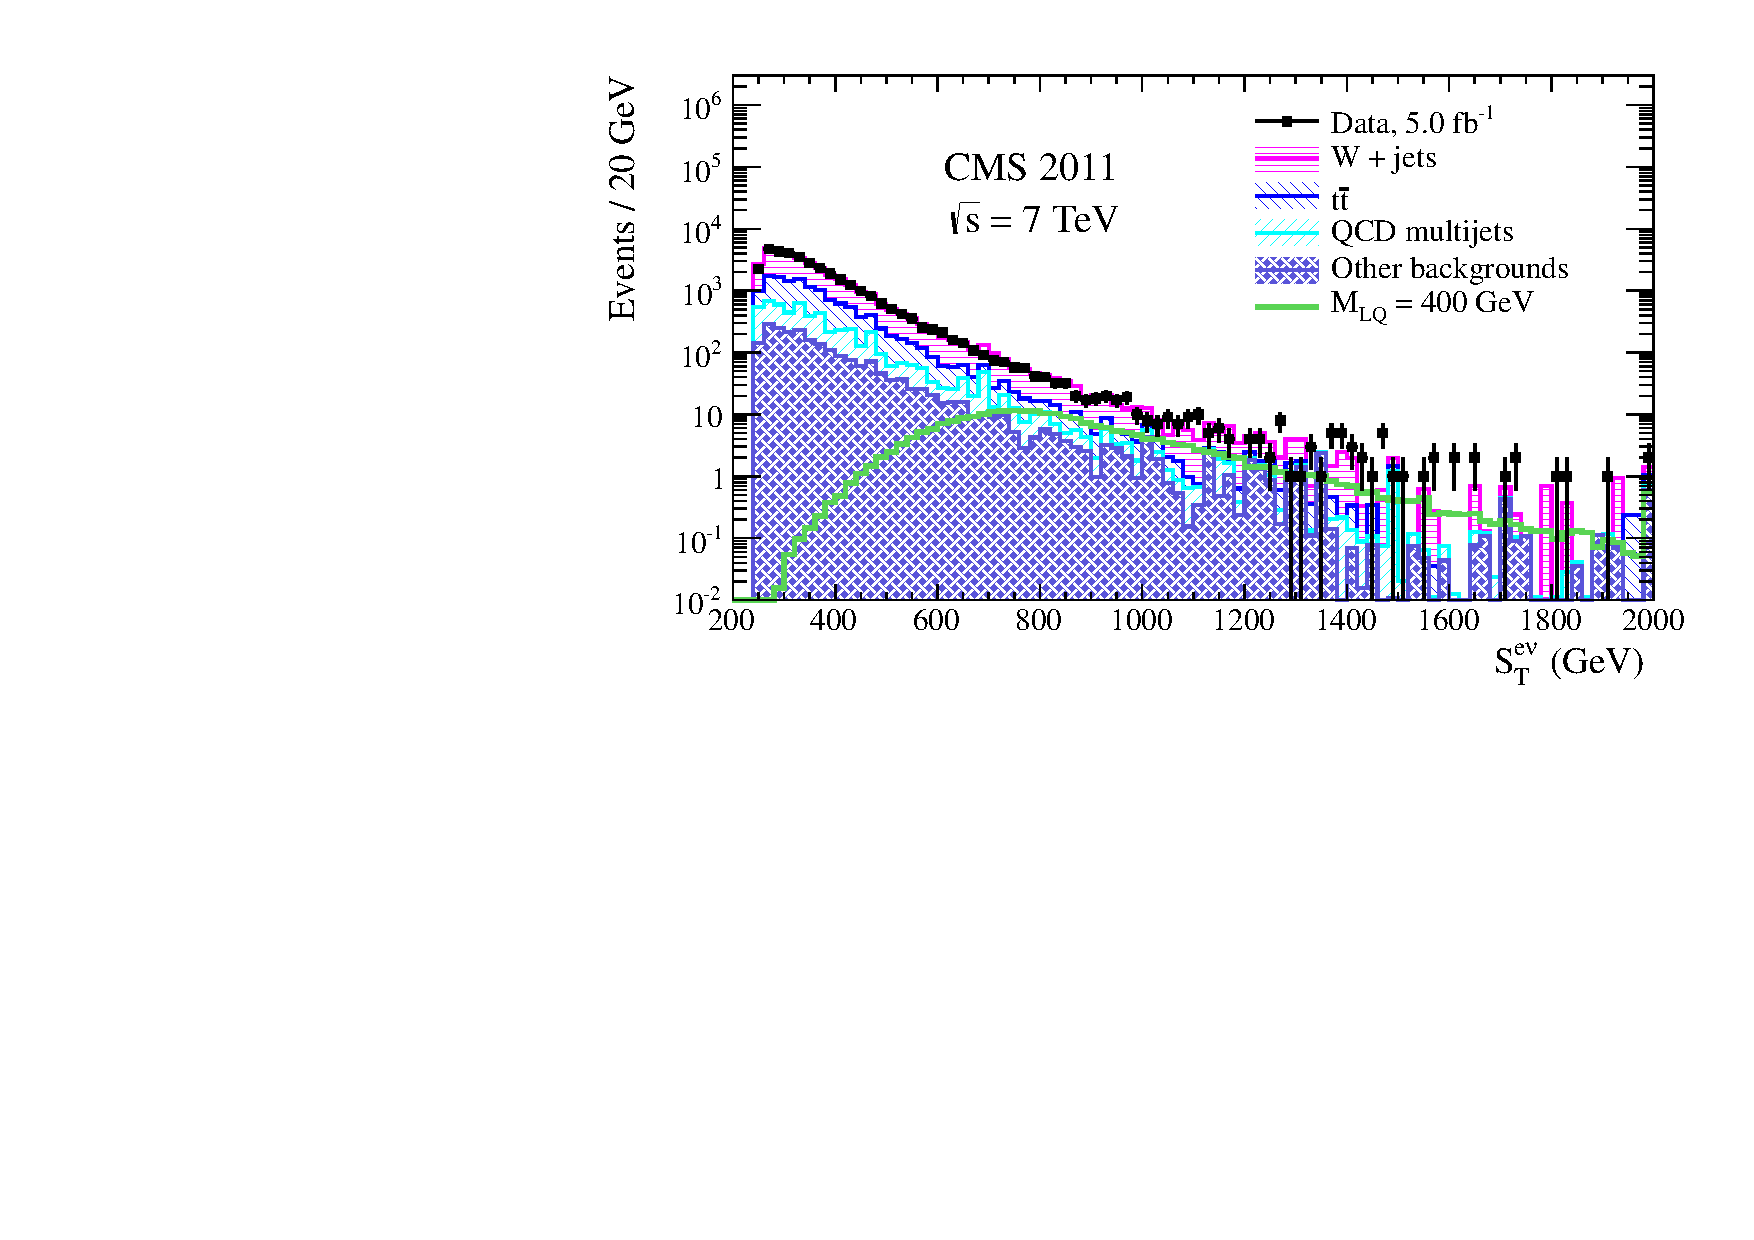
\includegraphics[width=.45\textwidth]{tex/analysis/event_selection/fig/enu/preselection/sT_PAS_enujj_WZSherpa_noNSigma.pdf}}
    \caption{
      The \mt (left) and \st (right) distributions for events passing the \enujj~preselection.
    }
    \label{fig:enujj_preselection_mt_and_st}
  \end{center}
\end{figure*}

\begin{figure*}[htbp]
  \begin{center}
    {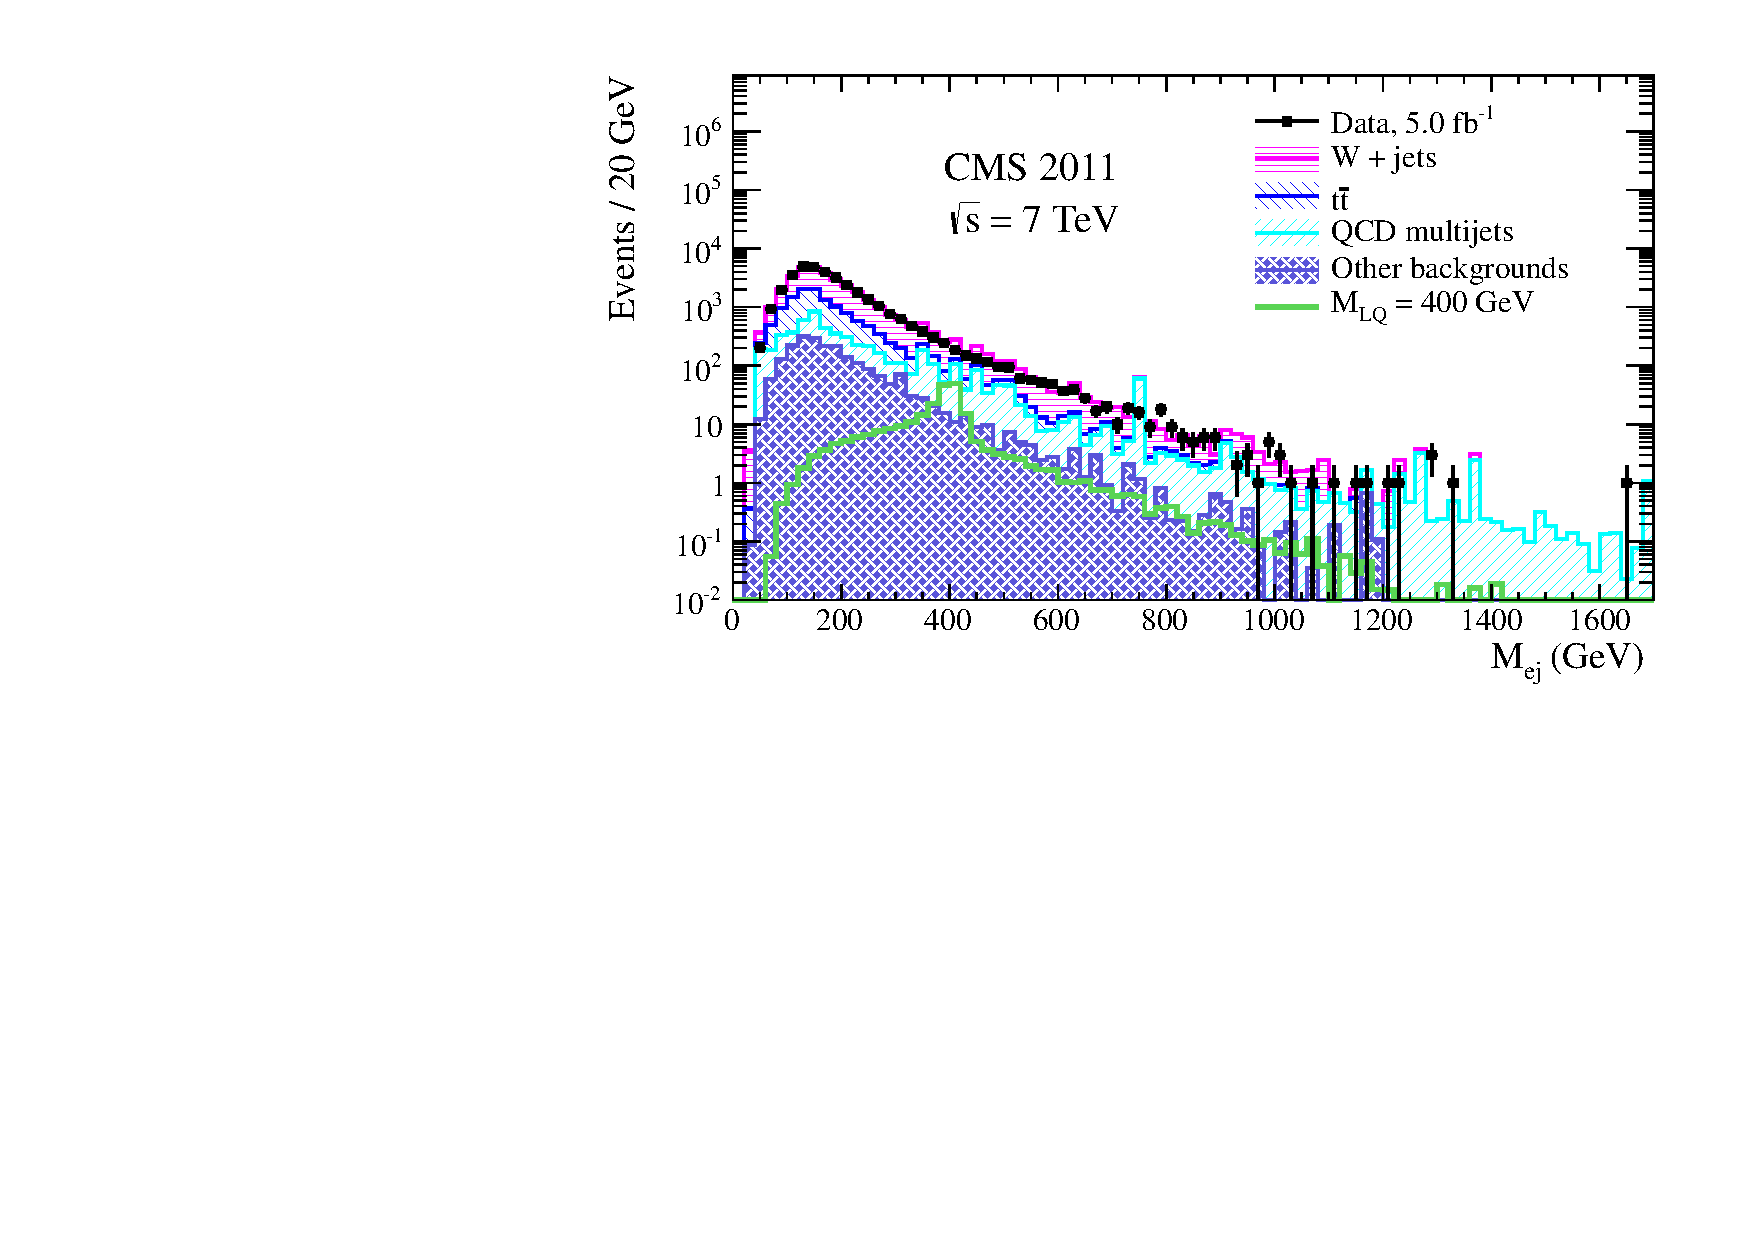
\includegraphics[width=.45\textwidth]{tex/analysis/event_selection/fig/enu/preselection/Mej_PAS_enujj_WZSherpa_noNSigma.pdf}}
    {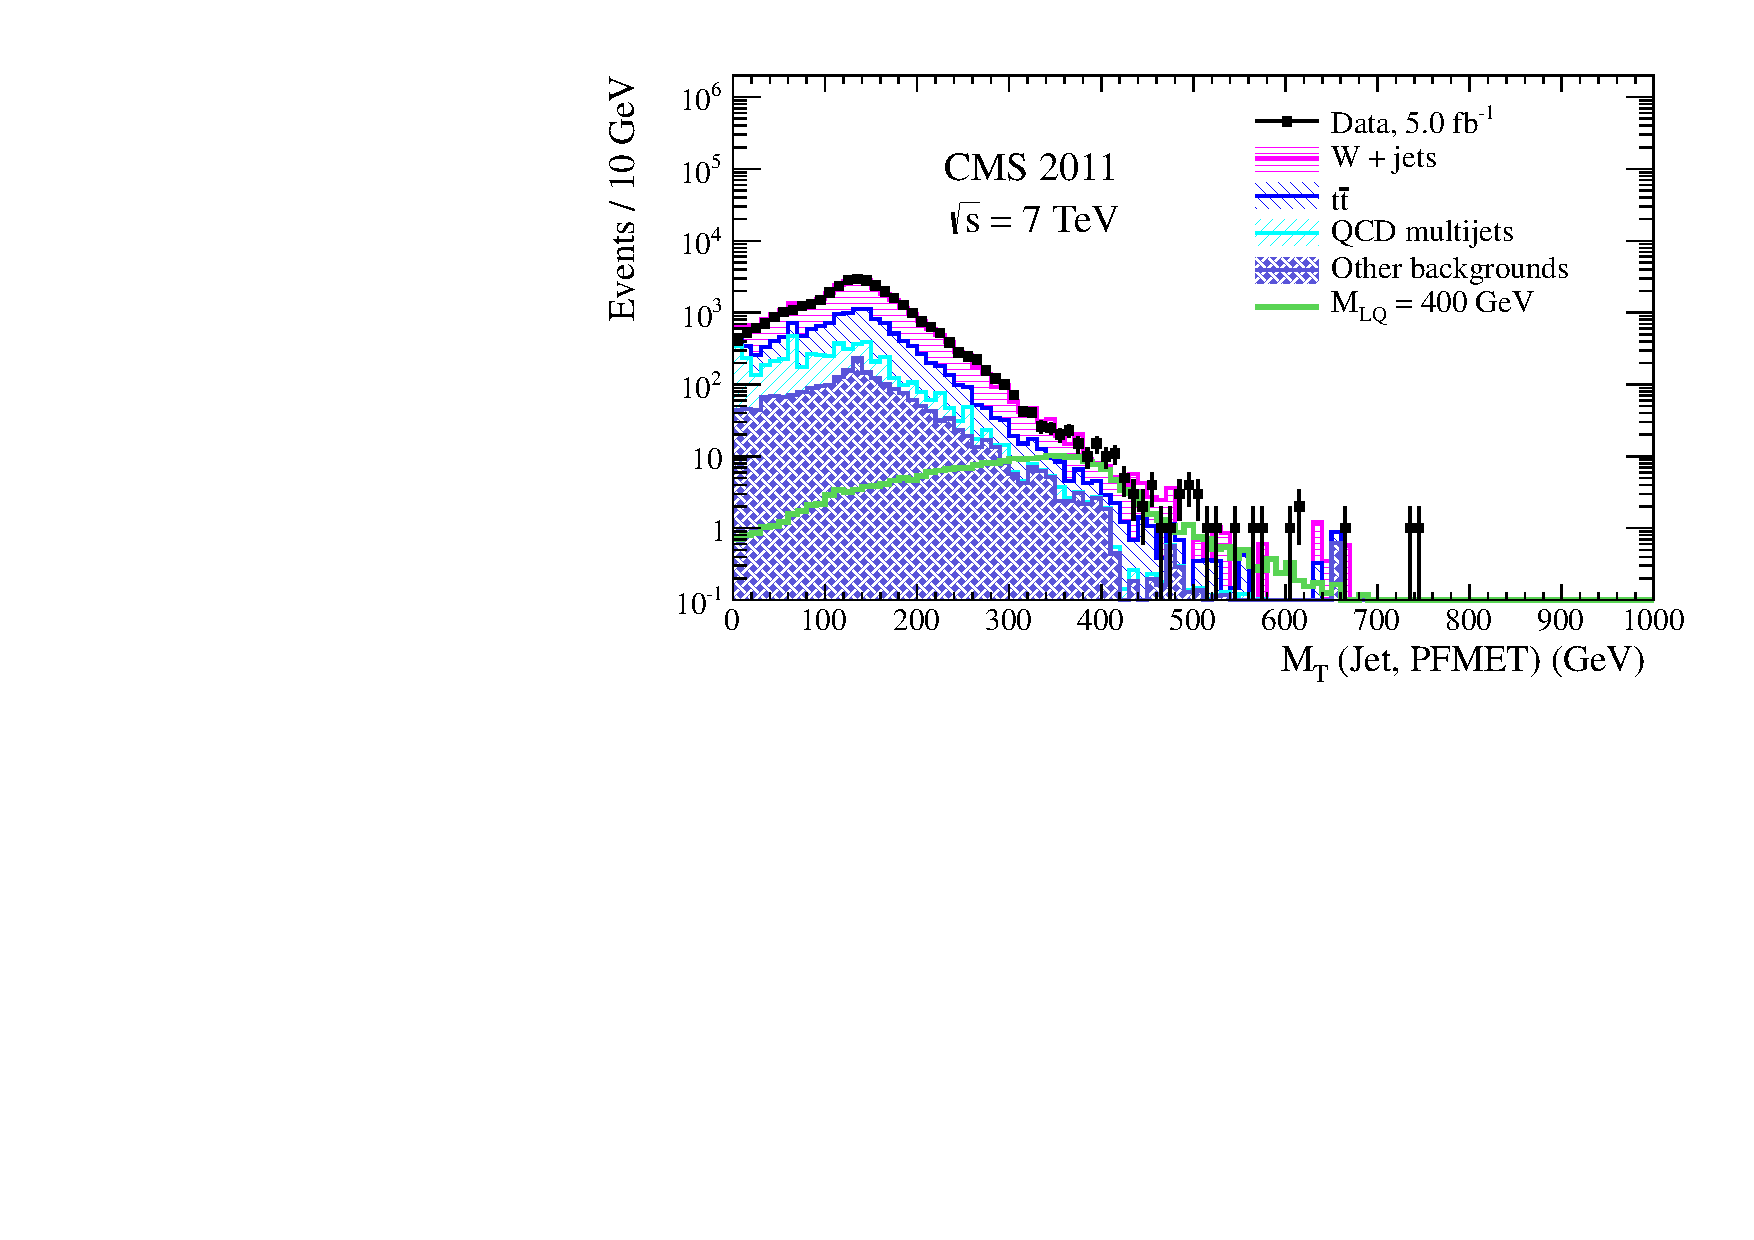
\includegraphics[width=.45\textwidth]{tex/analysis/event_selection/fig/enu/preselection/MTjnu_PAS_enujj_WZSherpa_noNSigma.pdf}}
    \caption{
      The \mej (left) and $m_{\text{T}\nu\text{j}}$ (right) distributions 
      for events passing the \enujj~preselection.
    }
    \label{fig:enujj_preselection_mej_and_mt}
  \end{center}
\end{figure*}


A sample of events enriched in SM background processes is 
selected to verify the background estimate in the \enujj~channel.
This \enujj~preselection proceeds with the following kinematics cuts
(all the reconstructed objects are required to pass the selection criteria 
described in Chapter~\ref{ch:analysis-object-selection}):
\begin{itemize}
\item Pass the event filters listed in Section \ref{sec:event-filters}
\item Pass the signal triggers listed in Table \ref{tab:enujjSingleEleElectronHadHLT} 
\item Exactly 1 HEEP electron with \pt$> 40$~\GeV and $|\eta| < 2.1$
\item At least 2 jets with \pt$>40$~\GeV and $|\eta|<2.4$
\item $\MET>55$ GeV
\item No selected muons passing the ID described in Section \ref{sec:id-muon}
\item \dphimetele$>0.8$; 
\item \dphimetjetone$>0.5$; 
\item \dRejets$>0.7$;
\item \st$>250$~\GeV
\end{itemize}

The $\pt$ cut on the electrons is chosen to be high
enough for the triggers listed in Table \ref{tab:eejjDoublePhotEleHLT}
to be fully efficient.  An additional $|\eta|$ cut is applied to the electrons
in order to reduce the contribution of QCD multijet events to the total background;
this cut has a negligable effect on the signal efficiency.
The $|\eta|$ cut on the jets rejects potential fake jets reconstructed from anomalous
signals in the HF ($|\eta| > 3.0$); this cut has a negligable impact on the leptoquark
signal efficiency.
The value of the \met~cut is set so that the signal triggers described in Table \ref{tab:enujjSingleEleElectronHadHLT} 
are fully efficient.
\dphimetele~and \dphimetjetone~are the opening angles between the \met~and the electron
and leading jet in \pt, respectively.  \dRejets~is the separation in $\Delta R$ between the
electron and the leading jet in \pt.
All three of these cuts were included to reduce the 
contribution of QCD multijet events to the total background, and the values were chosen
to have a negligable impact on the leptoquark signal efficiency.
The muon veto rejects backgrounds from \ttbar~events with an $e\mu jj$ final state.
The \st~cut is looser than the cuts applied in the final selection of the \enujj~channel.

At this stage of the selection, there is sufficient data to
compare with the background predictions for all the observables
employed in the final event selection.
The distribution of the number of reconstructed primary vertices is shown
in Figure
\ref{fig:enujj_preselection_vertices}.
The \pt~and $\eta$ distributions of the electron
and the two leading jets are shown in Figures
\ref{fig:enujj_preselection_ele1}, 
\ref{fig:enujj_preselection_jet1}, and  
\ref{fig:enujj_preselection_jet2}.
The \MET~distribution is shown in Figure
\ref{fig:enujj_preselection_met}.
The 
$\Delta\phi(\MET,\text{e})$, 
$\Delta\phi(\MET,\text{j1})$, 
$\Delta\phi(\MET,\text{j2})$, and 
$\text{min}\Delta R (\text{e},\text{jets})$ 
distributions are shown in Figure
\ref{fig:enujj_preselection_deltaPhi}.
The \mt~and \st~distributions are shown in Figure
\ref{fig:enujj_preselection_mt_and_st}.
The \mej~and $m_{\text{T}\nu\text{j}}$ distributions are shown in Figure
\ref{fig:enujj_preselection_mej_and_mt}.
